\documentclass[11pt]{article}

\usepackage[a4paper,margin=2.7cm]{geometry}
\usepackage{amsmath,amssymb,bm}
\usepackage{graphicx}
\usepackage{booktabs}
\usepackage{float}
\usepackage{tikz}
\usepackage[colorlinks=true,linkcolor=blue,citecolor=blue,urlcolor=blue]{hyperref}
\usetikzlibrary{positioning,fit,backgrounds,arrows.meta}

\newcommand{\vA}{v_{A}}
\newcommand{\vB}{v_{B}}

\title{Learning inter-family correlations with a shared hidden layer:\\
a two-family Ising model as a controlled test case}
\author{}
\date{}

\begin{document}
\maketitle

\begin{abstract}
We consider a toy statistical-mechanics system made of two weakly coupled
Ising subsystems (``families''), each with its own sparse random
intra-family couplings and a sparse set of inter-family couplings. We ask
whether a Restricted Boltzmann Machine (RBM), trained only on
family-resolved data, can be extended with a small number of additional
hidden units to recover the inter-family coupling structure without
disturbing what has already been learned about each family in isolation.
The extension is built by freezing the parameters of two independently
trained RBMs inside a larger, paired RBM and leaving only a block of newly
added hidden units, connected to the full joint visible layer, free to
adapt. These added units recover genuine cross-family structure: the
correlation matrix sampled from the trained paired model at equilibrium
correlates with the true coupling matrix at $r\approx0.84$, close to the
finite-sample ceiling set by the data themselves ($r\approx0.85$), and far
above the $r\approx0$ obtained from two independent, uncoupled RBMs. We
then scan the number of added units, trained long enough at a low enough
learning rate to reach full convergence at every size, and find a less
comfortable picture than a shorter, less careful sweep first suggested:
cross-family recovery saturates once roughly $20$--$30$ units are present,
but each family's own single-site statistics take a corresponding,
persistent hit once the added units start doing genuine cross-family work
-- one that does \emph{not} shrink again as more units are added, unlike
what under-trained large-capacity runs at a higher learning rate had
appeared to show.
\end{abstract}

\section{Motivation}

Many complex systems are not single homogeneous systems but collections
of weakly interacting subsystems: coupled spin lattices, interacting
neural populations, or correlated biological sequence families. A
recurring question in this setting is whether a genuine cross-subsystem
coupling can be identified from data, as opposed to a spurious
correlation induced by imperfectly estimated single-subsystem statistics.
We study this on a toy model where the answer is known by construction:
two Ising subsystems joined by a sparse matrix of inter-family couplings.
Rather than training a single RBM on the joint data, we train two
independent RBMs on each family alone, then add a small block of
\emph{additional} hidden units on top of the two frozen models to account
for whatever they fail to explain -- the inter-family correlations. This
isolates, quite literally, the channel through which the model can
represent cross-family information, so that channel's output can be
checked directly against the known ground truth.

\section{Model and data}
\label{sec:model}

Each family $X\in\{A,B\}$ consists of $N=30$ Ising spins $s_i^X=\pm1$. The
joint system of $60$ spins is governed by
\begin{equation}
\mathcal{H}(\bm{s}_A,\bm{s}_B) = -\sum_{i<j} J^A_{ij}\,s^A_i s^A_j
-\sum_{i<j} J^B_{ij}\,s^B_i s^B_j
-\sum_{i,j} K_{ij}\,s^A_i s^B_j
-\sum_i h^A_i s^A_i -\sum_i h^B_i s^B_i \, ,
\label{eq:hamiltonian}
\end{equation}
sampled at inverse temperature $\beta=0.5$ by single-spin-flip
Metropolis--Hastings, with $5000$ sweeps of burn-in and $100$ sweeps of
thinning between the $20\,000$ recorded configurations ($70/15/15$
train/validation/test split). The intra-family couplings $J^A,J^B$ sit on
sparse random graphs (edge density $0.12$, $J\in[-0.8,0.8]$); the
inter-family coupling $K$ is sparser still, $100$ non-zero entries out of
$900$ possible pairs ($11\%$ density), $K\in[-0.9,0.9]$. The local fields
are drawn from $h\in[-0.3,0.3]$ -- wide enough that each site's marginal
$\langle s_i\rangle$ carries a signal well above the sampling noise of the
diagnostics used below (Section~\ref{sec:hadd-sweep} discusses why this
matters). No information about $J^A$, $J^B$ or $K$ is passed to the
learning stage.

\section{RBM architecture and the paired construction}
\label{sec:paired}

We use a Potts RBM: visible units are one-hot, $q=2$-state variables (the
natural generalisation of an Ising spin), paired with hidden units of the
\emph{xReLU} family (a continuous, dReLU-type response with unbounded
asymmetry). Training is by Persistent Contrastive Divergence -- persistent
Monte Carlo chains advanced $50$ sweeps between successive Adam updates
($\beta_1=0$, $\beta_2=0.999$, learning rate $10^{-4}$), batch size $512$
-- for $20\,000$ steps per private RBM ($30$ hidden units each).

The \emph{paired} model (Fig.~\ref{fig:architecture}) concatenates the two
families' visible layers ($60$ spins) and the two private hidden layers,
plus $H_{\mathrm{add}}$ newly added hidden units. The private $A$--$A$ and
$B$--$B$ weight blocks are initialised from the independently trained
RBMs and then \emph{frozen}: after every gradient step, they are reset to
their reference values, discarding whatever update the optimiser proposed.
The cross blocks ($A$'s hidden units to $B$'s visible units, and vice
versa) are pinned at exactly zero throughout. The only free parameters are
the added units' weights to the full $60$-spin visible layer and their own
biases -- trained for a further $10\,000$ steps, with the raw gradient's
global norm clipped to $1$ before every Adam update (Section~\ref{sec:results}
discusses why this is necessary at this learning rate and step count). By
construction, any cross-family dependence the paired model can represent
must flow through these added units.

\begin{figure}[H]
\centering
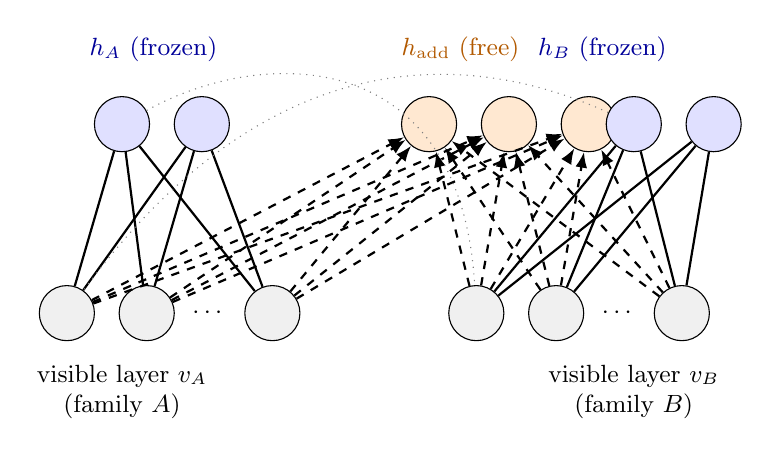
\begin{tikzpicture}[
  node distance=10mm,
  unit/.style={circle, draw, minimum size=7mm, inner sep=0pt},
  frozen/.style={unit, fill=blue!12},
  addedu/.style={unit, fill=orange!18},
  visu/.style={unit, fill=gray!12},
  frozenedge/.style={draw, thick},
  freeedge/.style={draw, thick, dashed, -{Latex[length=2mm]}},
  zeroedge/.style={draw, thin, dotted, gray},
  font=\small
]
  \node[visu] (vA1) at (0,0) {};
  \node[visu] (vA2) [right=3mm of vA1] {};
  \node (vAdots) [right=1mm of vA2] {$\cdots$};
  \node[visu] (vA3) [right=1mm of vAdots] {};
  \node[visu] (vB1) at (5.2,0) {};
  \node[visu] (vB2) [right=3mm of vB1] {};
  \node (vBdots) [right=1mm of vB2] {$\cdots$};
  \node[visu] (vB3) [right=1mm of vBdots] {};

  \node[frozen] (hA1) at (0.7,2.4) {};
  \node[frozen] (hA2) [right=3mm of hA1] {};
  \node[addedu] (hadd1) at (4.6,2.4) {};
  \node[addedu] (hadd2) [right=3mm of hadd1] {};
  \node[addedu] (hadd3) [right=3mm of hadd2] {};
  \node[frozen] (hB1) at (7.2,2.4) {};
  \node[frozen] (hB2) [right=3mm of hB1] {};

  \foreach \h in {hA1,hA2}
    \foreach \v in {vA1,vA2,vA3}
      \draw[frozenedge] (\v) -- (\h);
  \foreach \h in {hB1,hB2}
    \foreach \v in {vB1,vB2,vB3}
      \draw[frozenedge] (\v) -- (\h);
  \foreach \h in {hadd1,hadd2,hadd3}
    \foreach \v in {vA1,vA2,vA3,vB1,vB2,vB3}
      \draw[freeedge] (\v) -- (\h);
  \draw[zeroedge] (hA1) .. controls (2.5,3.4) and (5.0,3.4) .. (vB1);
  \draw[zeroedge] (hB1) .. controls (5.0,3.4) and (2.5,3.4) .. (vA1);

  \node[align=center] at (0.7,-1.0) {visible layer $\vA$\\(family $A$)};
  \node[align=center] at (7.2,-1.0) {visible layer $\vB$\\(family $B$)};
  \node[align=center,text=blue!60!black] at (1.1,3.35) {$h_A$ (frozen)};
  \node[align=center,text=blue!60!black] at (6.8,3.35) {$h_B$ (frozen)};
  \node[align=center,text=orange!70!black] at (5.0,3.35) {$h_{\mathrm{add}}$ (free)};
\end{tikzpicture}
\caption{Architecture of the paired RBM. Solid: private $A$--$A$/$B$--$B$
blocks, frozen at the independently trained values. Dotted: cross blocks
$h_A$--$\vB$, $h_B$--$\vA$, pinned at zero. Dashed: the only free
parameters, connecting the added units to the full visible layer.}
\label{fig:architecture}
\end{figure}

\section{Diagnostics}
\label{sec:diagnostics}

Training-time diagnostics compare data- and model-averaged moments along
the same short persistent chains used for the gradient -- cheap, but not a
substitute for equilibrium, since those chains are not guaranteed to be
mixed. The decisive test is performed after training: $5000$ independent
Gibbs chains, each run for $5000$ sweeps from the visible layer's own
marginal, used to estimate the model's cross-family correlation
$\langle s_i^As_j^B\rangle$ and compare it against the true $K$, both by
the fraction of the $100$ strongest true couplings recovered among the
model's own $100$ strongest (``top-$K$ overlap'') and by the whole-matrix
Pearson correlation with $K$. Both are also computed for the training data
themselves (a finite-sample ceiling, since $K$ is sparse enough that even
a perfect model cannot reach $r=1$ against it) and for a null model of two
independent, uncoupled RBMs (zero learned coupling).

\section{Results: $H_{\mathrm{add}}=30$}
\label{sec:results}

We first look in detail at one representative configuration,
$H_{\mathrm{add}}=30$ with training seed $5$ (chosen, among the $10$ seeds
run at this $H_{\mathrm{add}}$, for a particularly clean and legible
pseudo-likelihood trace), before scanning $H_{\mathrm{add}}$ itself in
Section~\ref{sec:hadd-sweep}.

\begin{figure}[H]
\centering
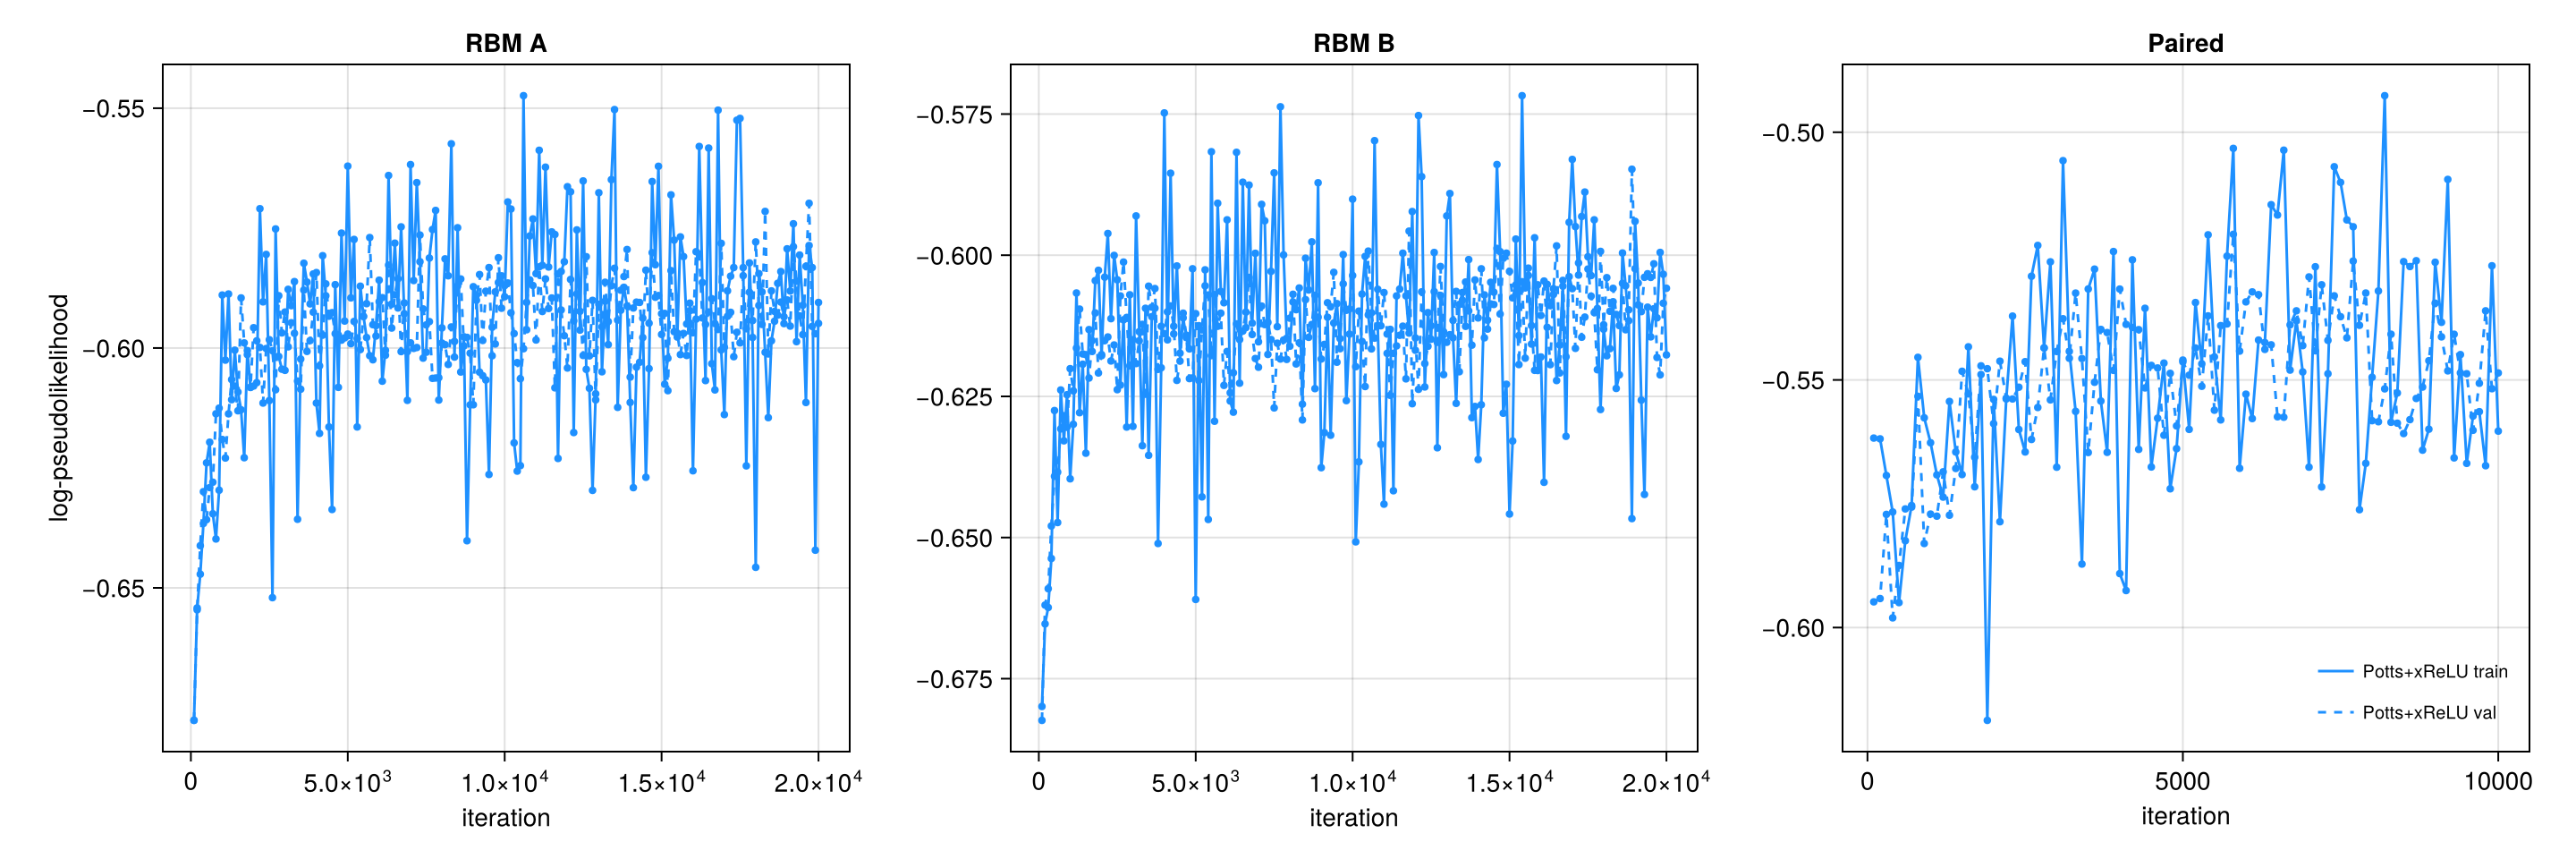
\includegraphics[width=0.75\linewidth]{figures/pseudolikelihood.png}
\caption{Training/validation pseudo-likelihood of the private RBMs and the
paired RBM, vs.\ gradient step.}
\label{fig:training}
\end{figure}

Pseudo-likelihood rises steadily and tracks its validation value closely
for both families and for the paired model (no overfitting;
Fig.~\ref{fig:training}). Fig.~\ref{fig:vhcheck} shows the corresponding
training-time hidden-unit activation alignment: both private RBMs stay
close to $r\approx0.95$ throughout, while the added units' alignment with
their own (short, unequilibrated) chains \emph{improves} over the course
of paired training, from $r\approx0.90$ to $r\approx0.995$. The
complementary check on single-site visible marginals
(Fig.~\ref{fig:vcheck}) tells the opposite story for the paired model: its
$\langle v\rangle$ alignment \emph{degrades} as training proceeds, from
$r\approx0.85$ to $r\approx0.3$--$0.5$, even as the private RBMs' own
$\langle v\rangle$ alignment stays flat around $r\approx0.75$--$0.85$
throughout. This is the training-time signature of the same collateral
effect quantified at equilibrium below and studied systematically in
Section~\ref{sec:hadd-sweep}.

\begin{figure}[H]
\centering
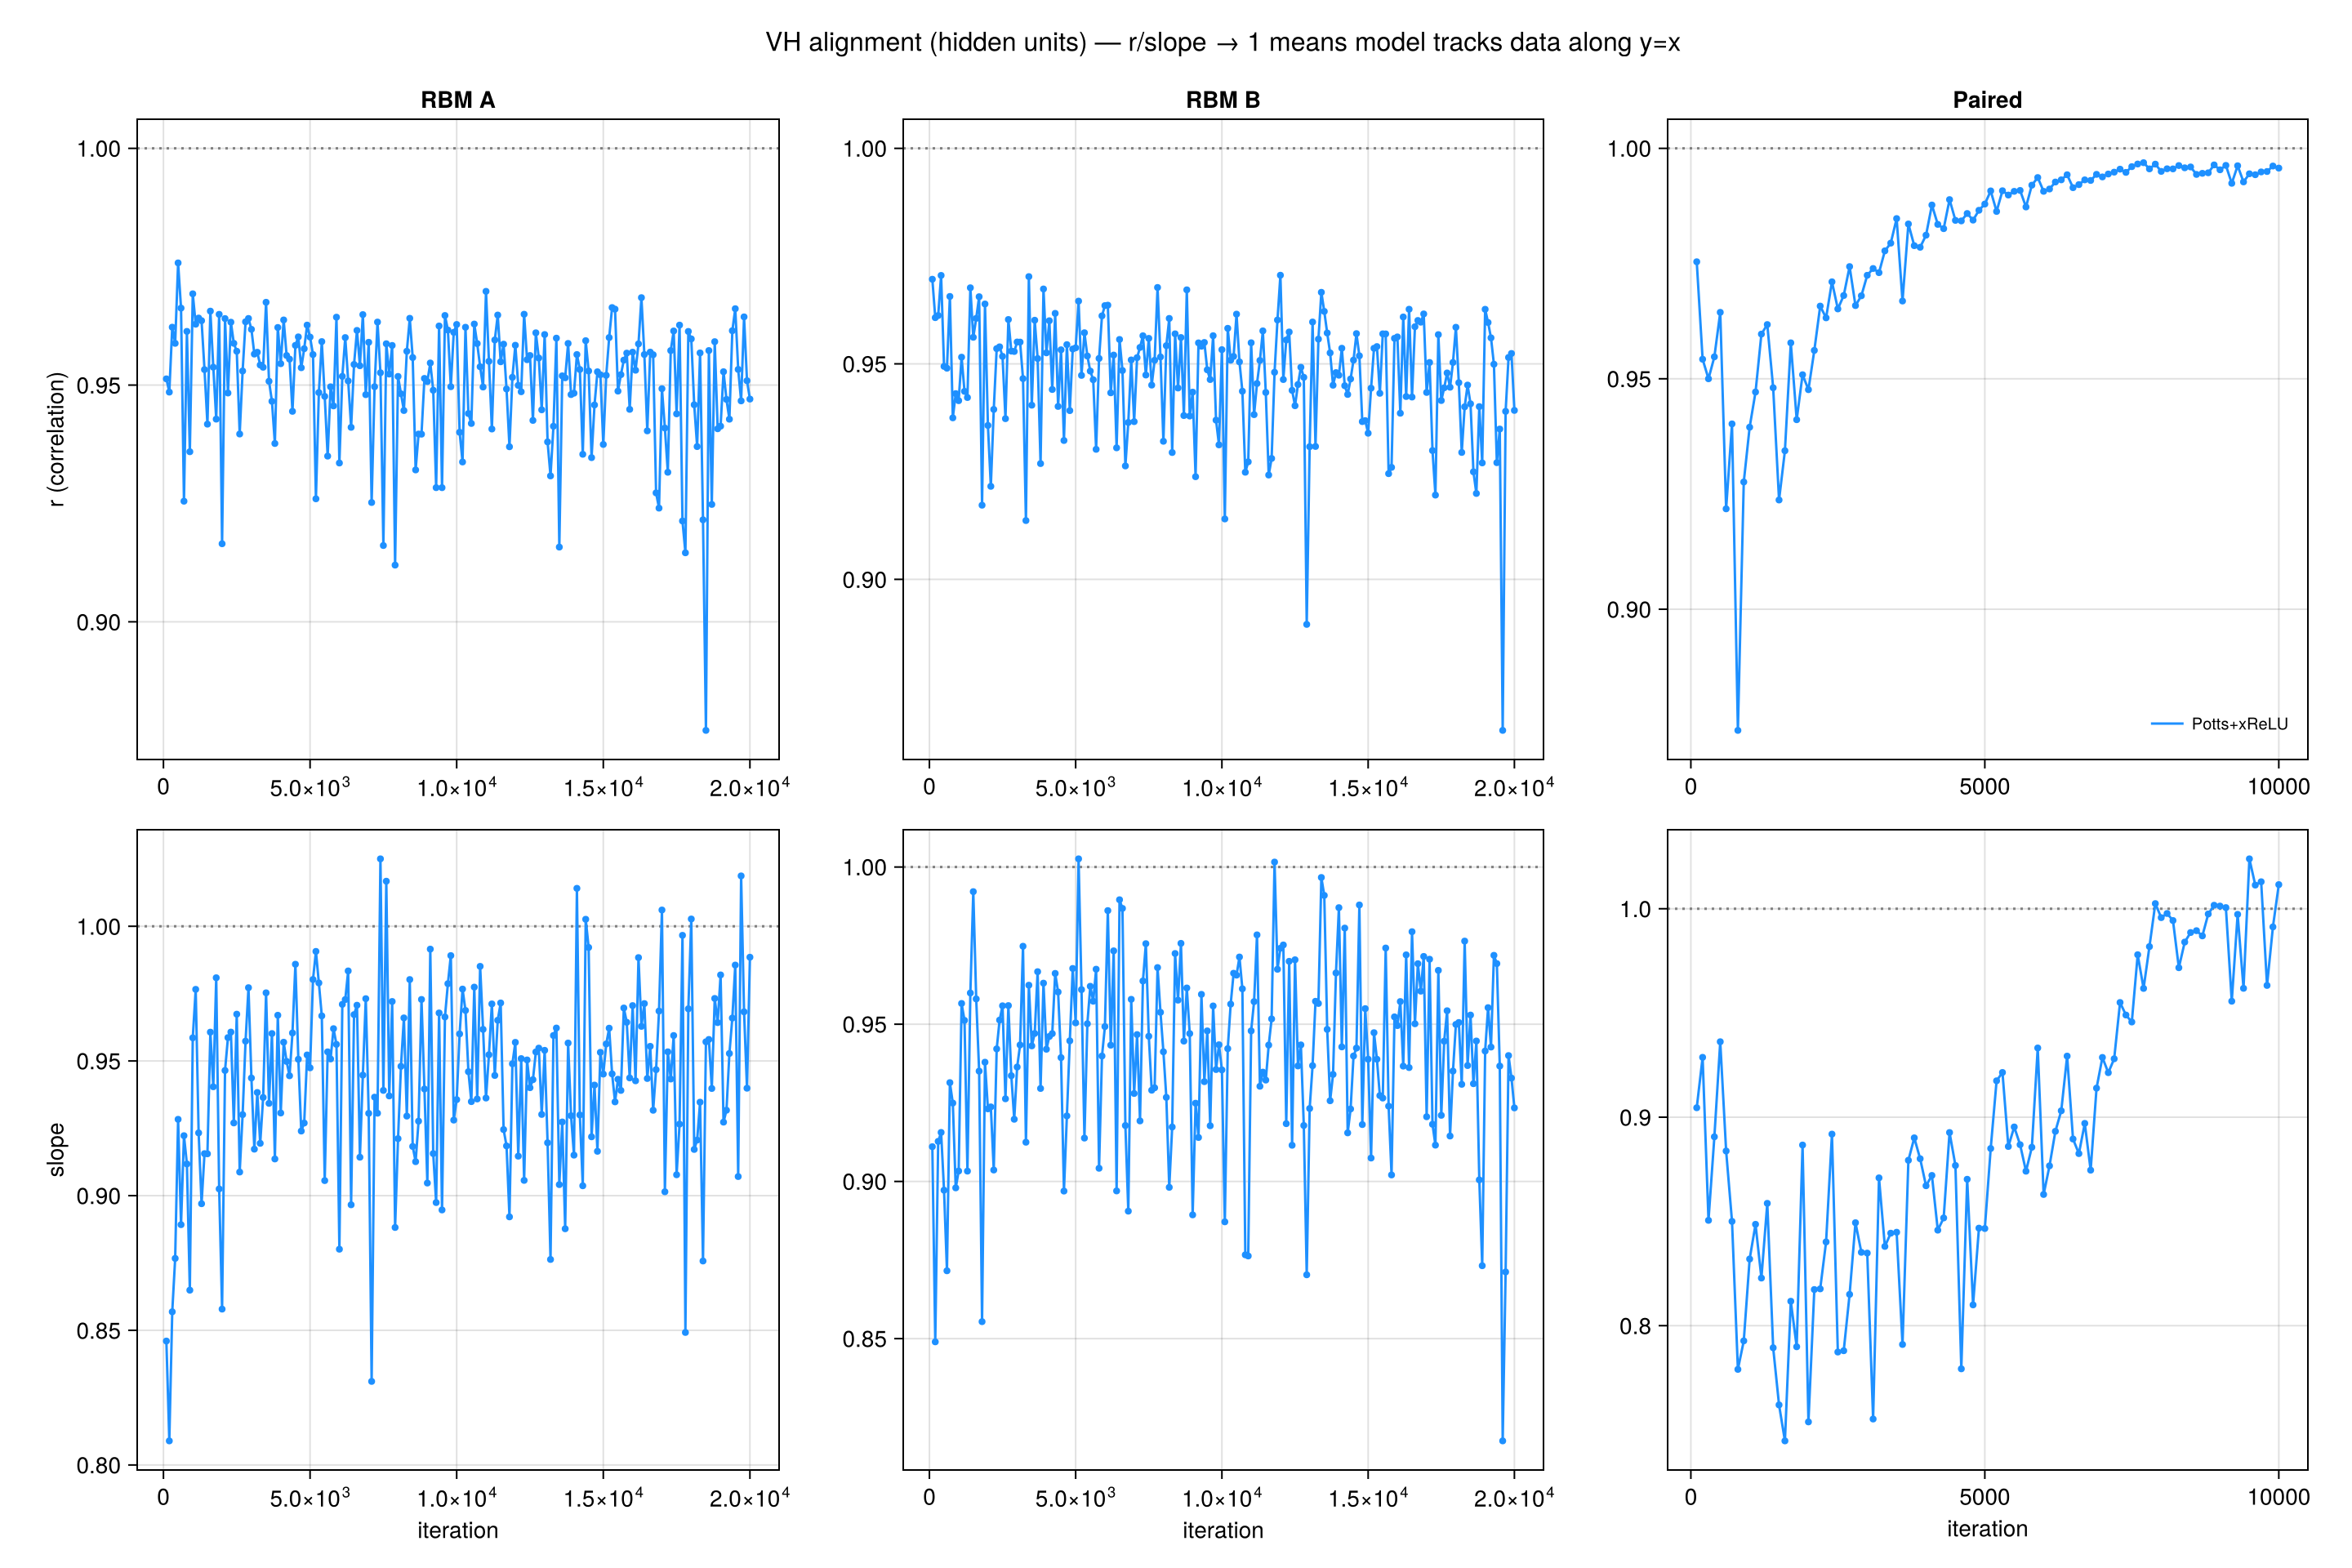
\includegraphics[width=0.85\linewidth]{figures/vh_check.png}
\caption{Training-time alignment (correlation $r$ and regression slope,
data vs.\ model) of hidden-unit activations $\langle hv\rangle$, vs.\
paired-training step for the added units (right column) and gradient step
for the private RBMs (left, middle columns).}
\label{fig:vhcheck}
\end{figure}

\begin{figure}[H]
\centering
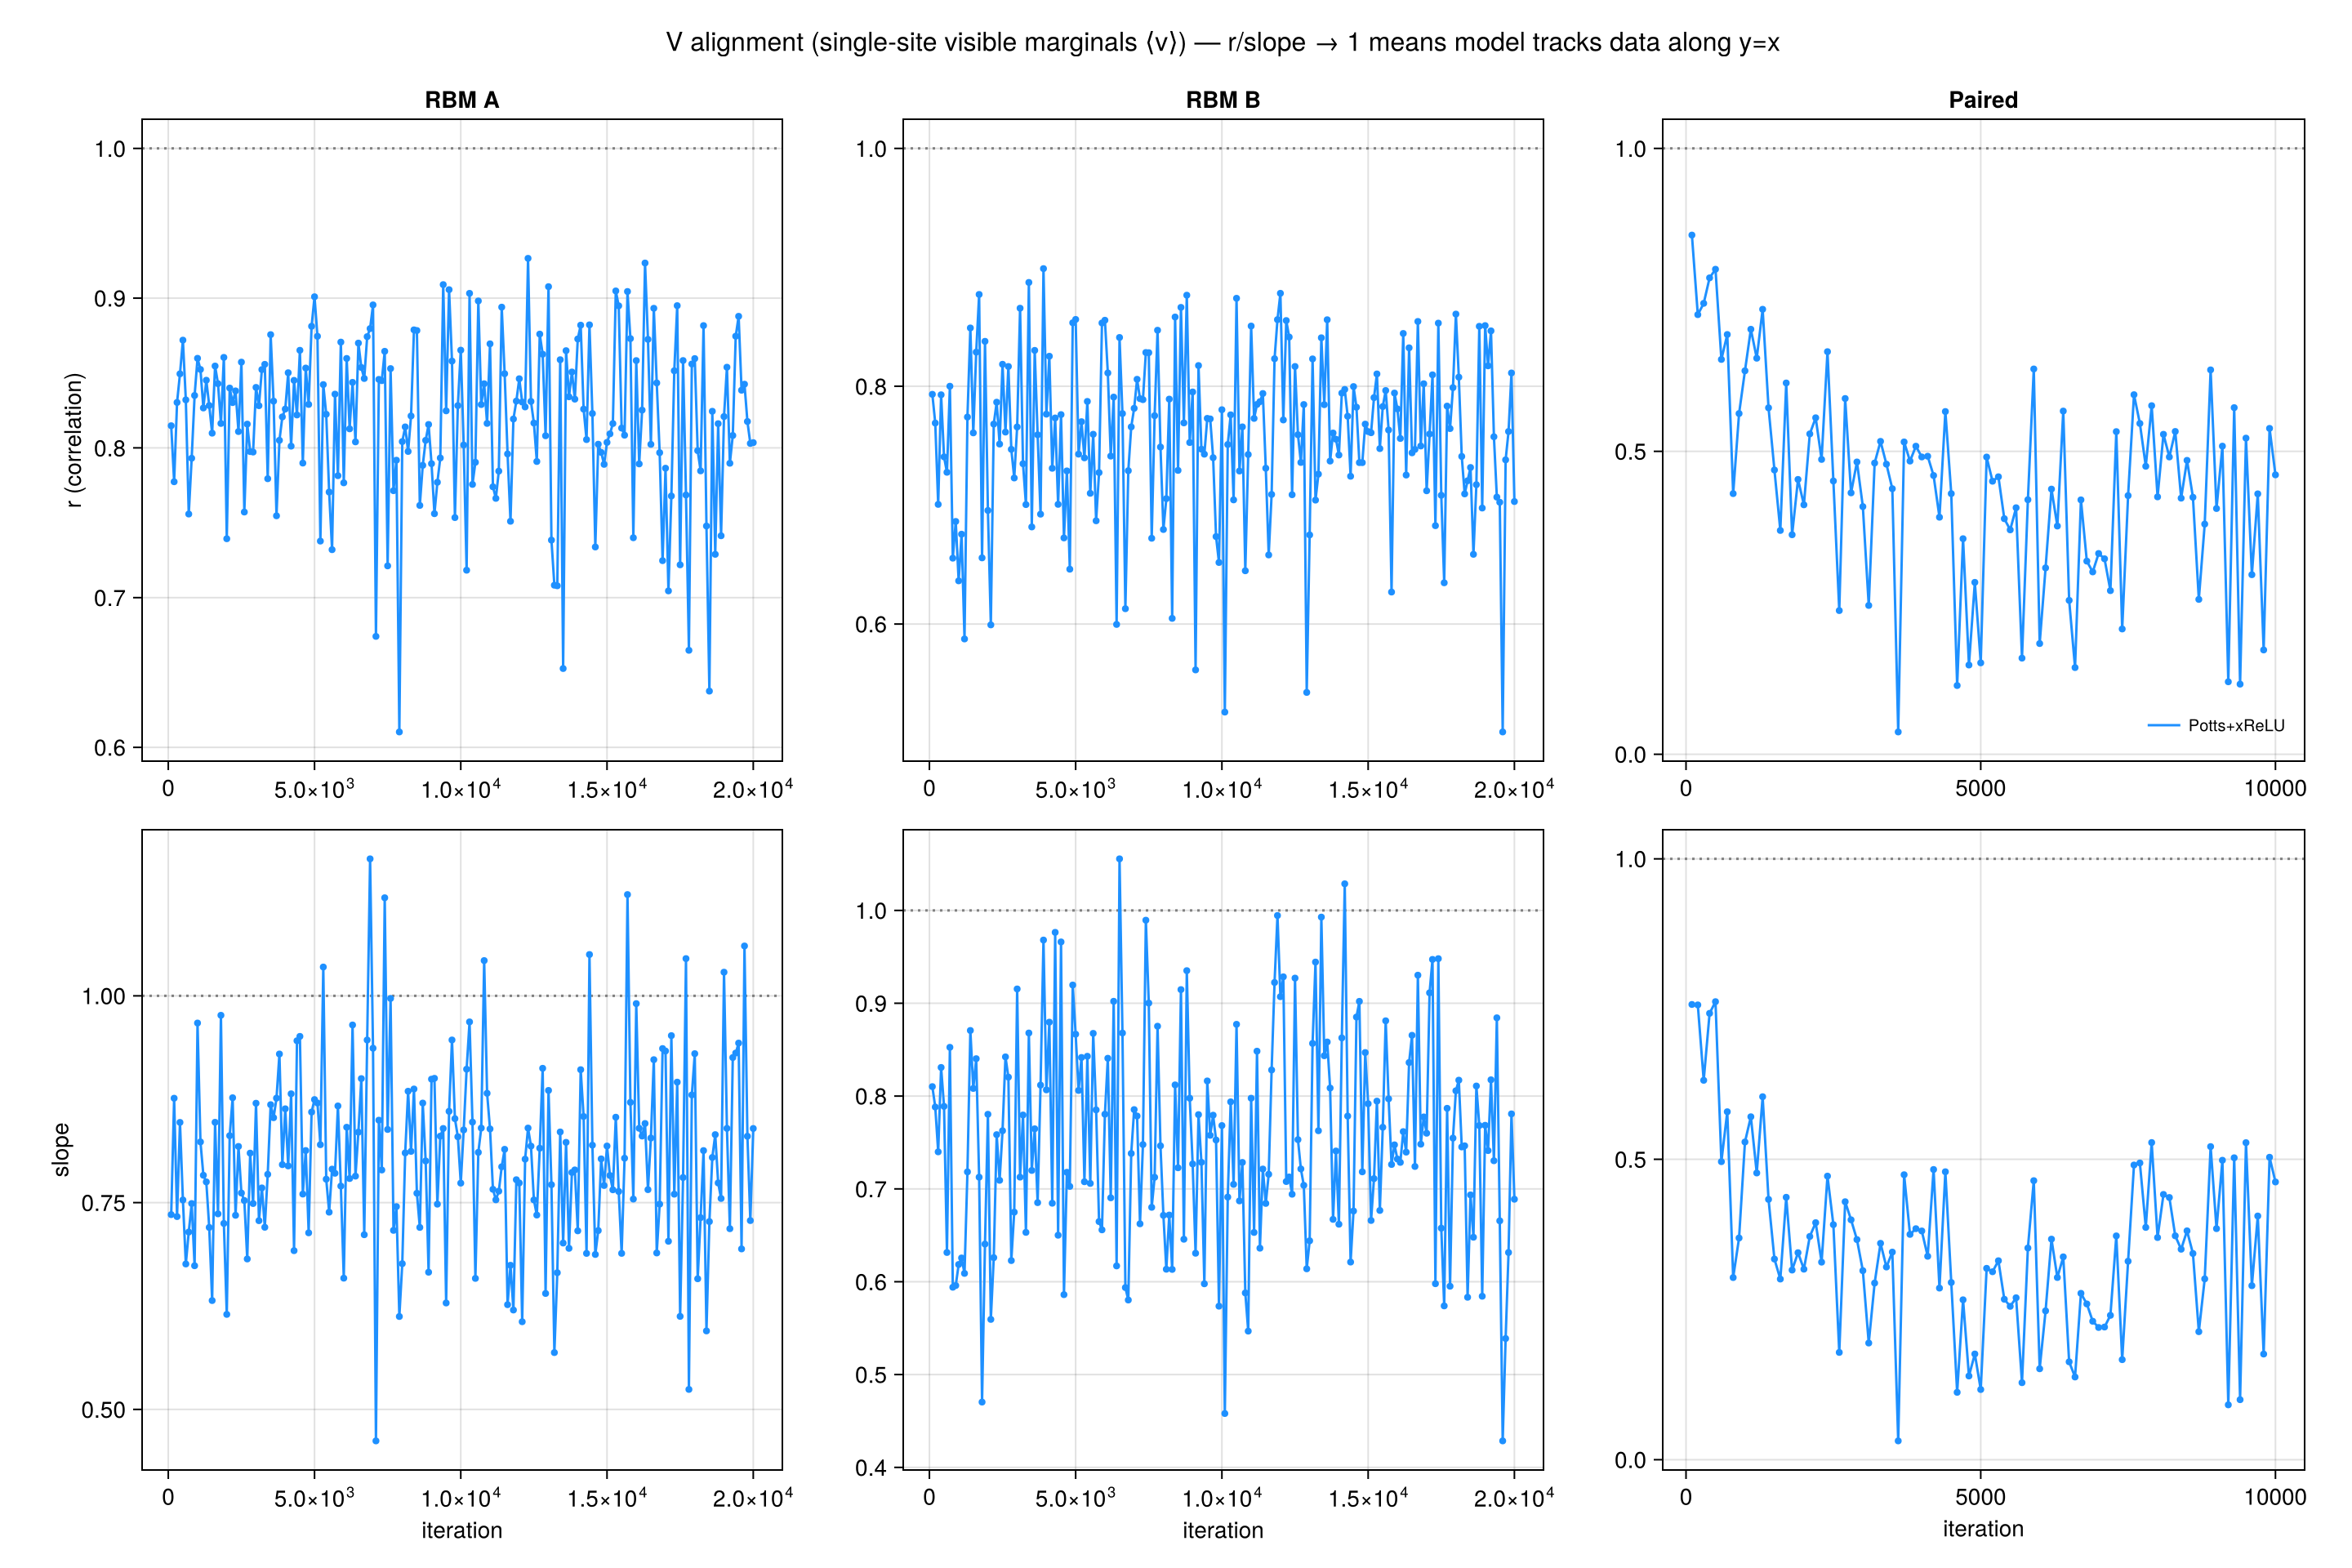
\includegraphics[width=0.85\linewidth]{figures/v_check.png}
\caption{Training-time alignment of single-site visible marginals
$\langle v\rangle$, same layout as Fig.~\ref{fig:vhcheck}. The paired
model's own alignment (right column) degrades as training proceeds,
opposite to Fig.~\ref{fig:vhcheck}.}
\label{fig:vcheck}
\end{figure}

The freeze check confirms the private blocks are untouched at every
logged step of paired training. The training-time interfamily correlation
check ($\langle v_i^Av_j^B\rangle$, data vs.\ model, Fig.~\ref{fig:abcheck}
left) climbs from $r\approx0.25$ to a stable $r\approx0.80$ over the
$10\,000$ paired steps -- encouraging, but measured on short,
unequilibrated chains and not yet the decisive test.

\begin{figure}[H]
\centering
\begin{minipage}[t]{0.48\linewidth}
\centering
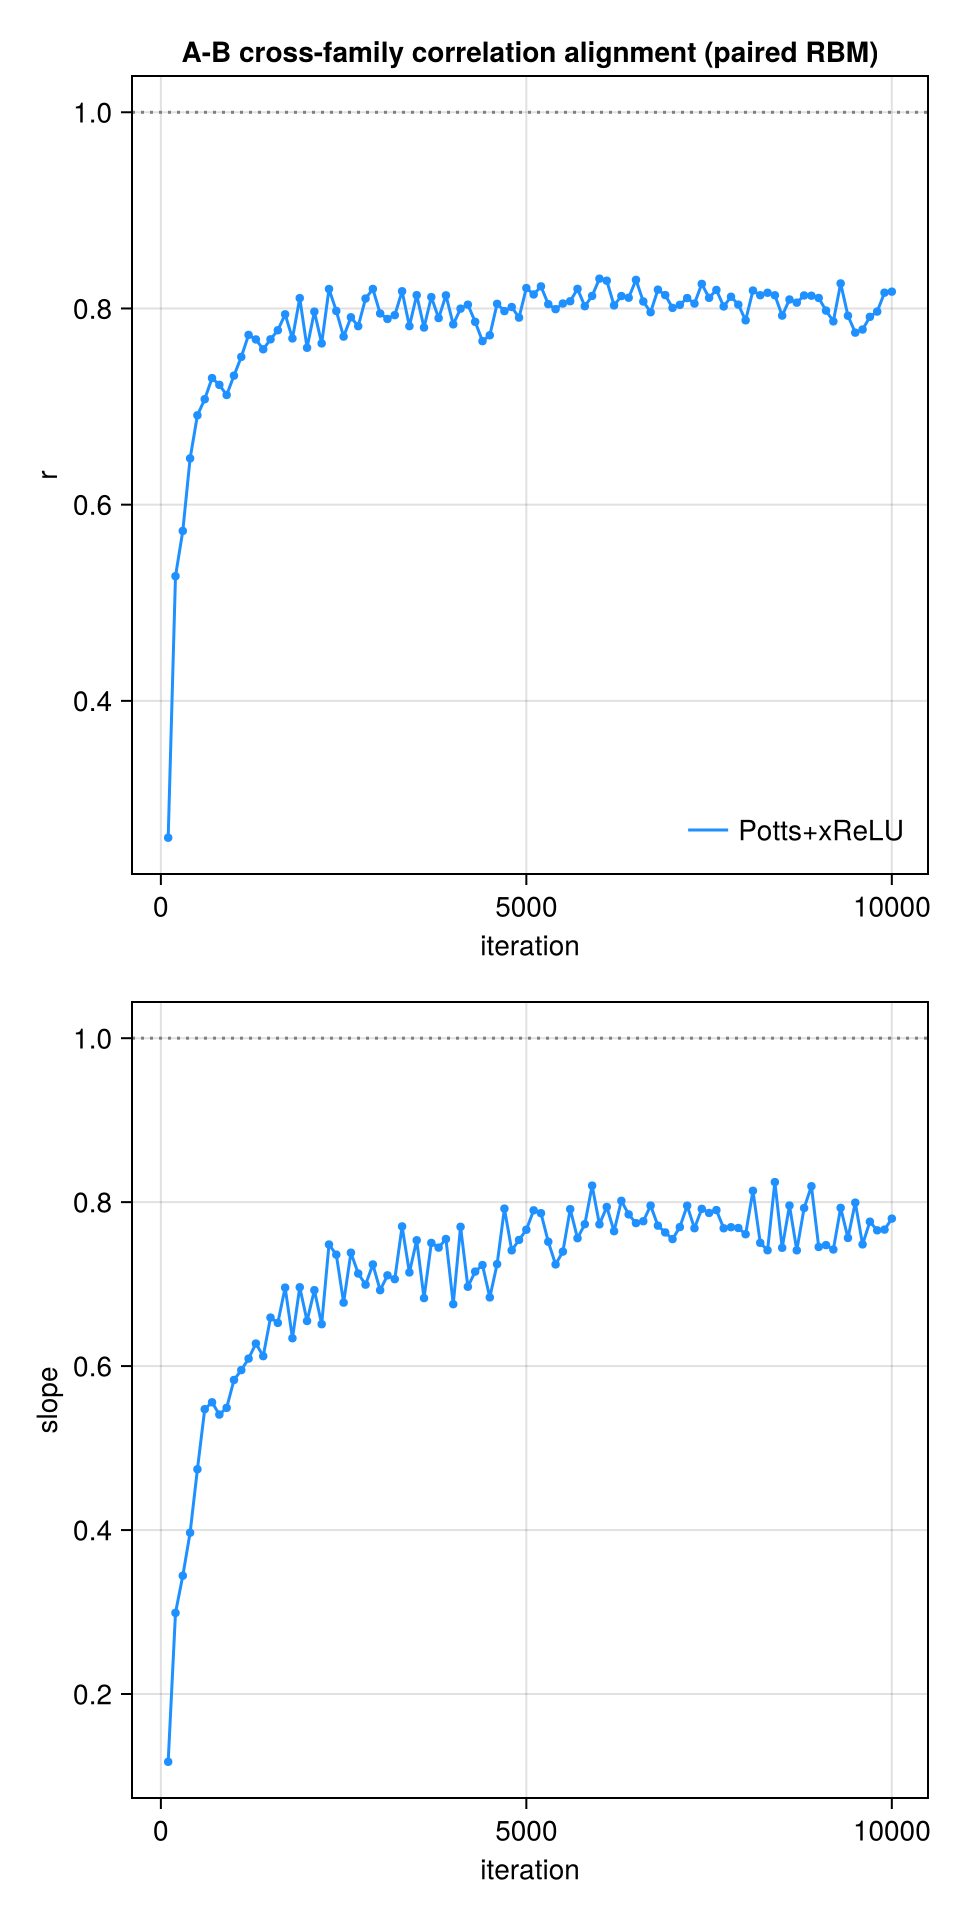
\includegraphics[width=\linewidth]{figures/ab_check_training.png}
\end{minipage}\hfill
\begin{minipage}[t]{0.48\linewidth}
\centering
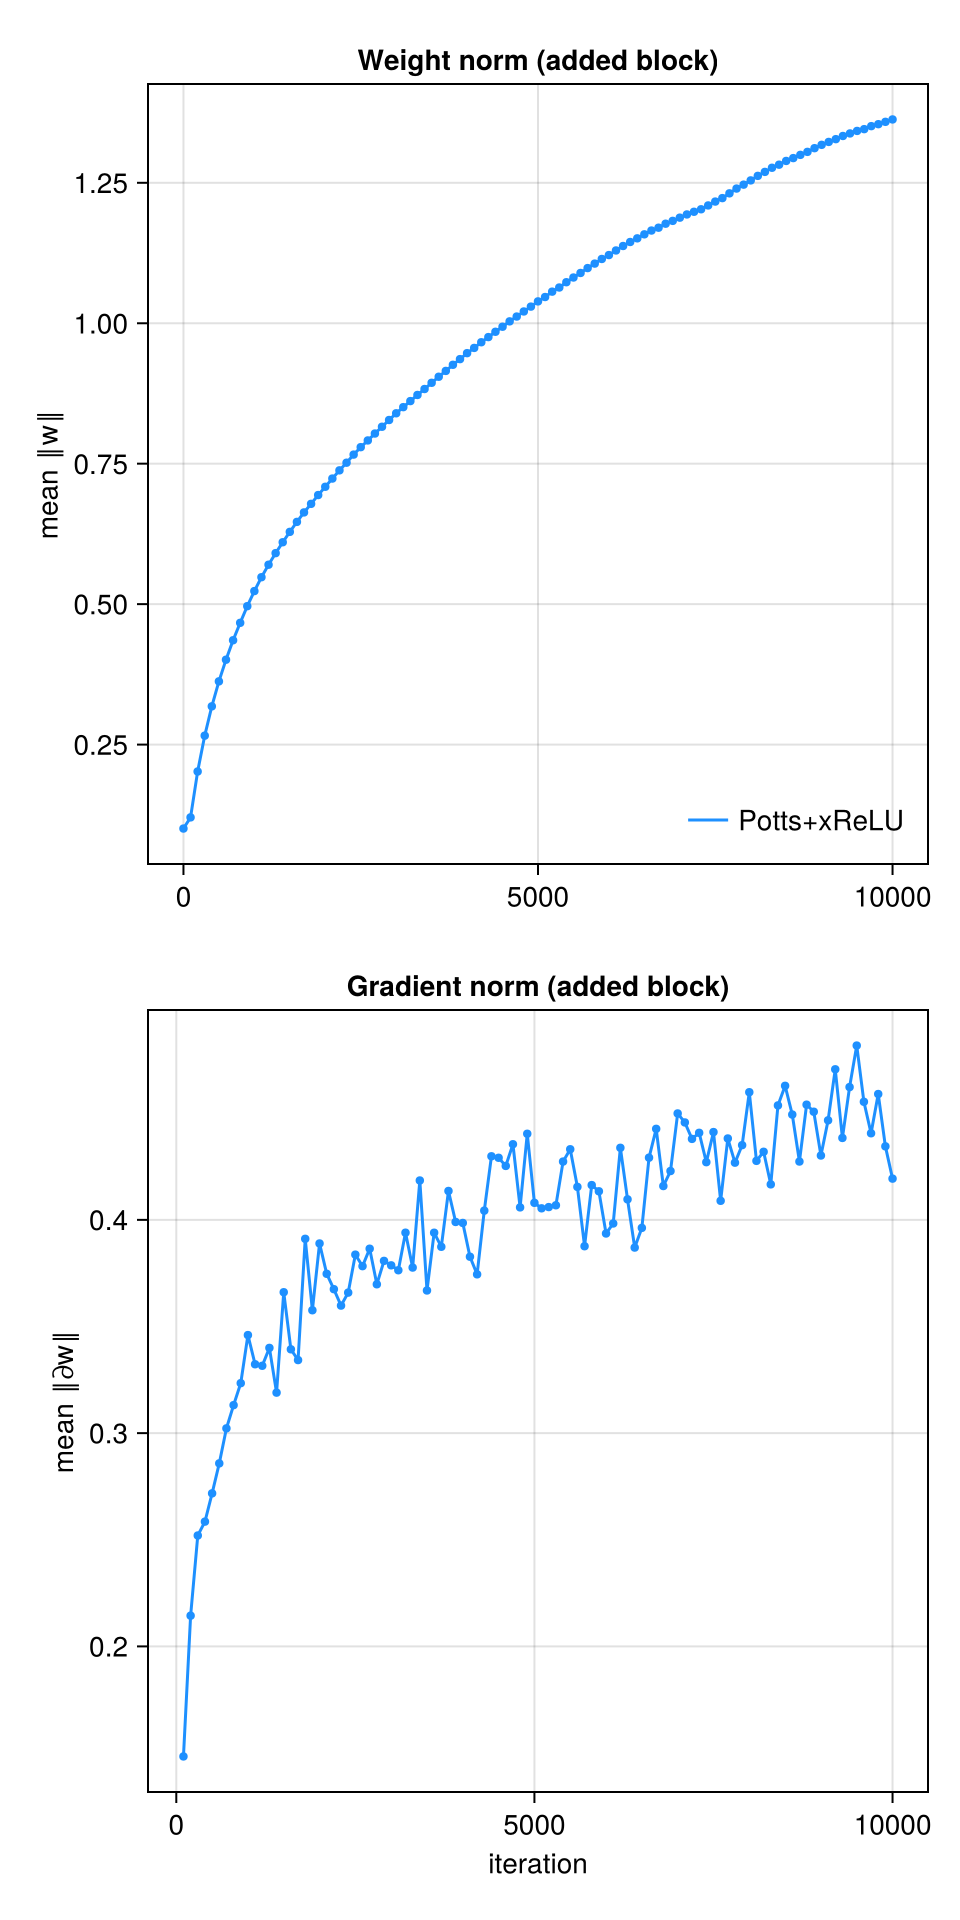
\includegraphics[width=\linewidth]{figures/norms_added_block.png}
\end{minipage}
\caption{Left: training-time $A$--$B$ cross-family correlation alignment
of the paired model. Right: mean weight norm and gradient norm of the
added-unit block over paired training. With gradient-norm clipping
(Section~\ref{sec:paired}), both grow smoothly and saturate; without it,
the same $10\,000$-step, learning-rate-$10^{-4}$ combination produced a
late-training runaway in $54$ of the $80$ swept configurations (weight
norm mean $2.3\to14.4$, max $4.3\to95.9$, over the last $\sim\!900$ steps,
with pseudo-likelihood collapsing in step) -- a single large gradient
spike late in training, which the slow-moving ($\beta_2=0.999$) second-moment
estimate cannot absorb quickly enough. The affected runs were archived and
all were successfully retrained with clipping; every one of the $80$
configurations reported here is clipping-stabilised and collapse-free.}
\label{fig:abcheck}
\end{figure}

\begin{figure}[H]
\centering
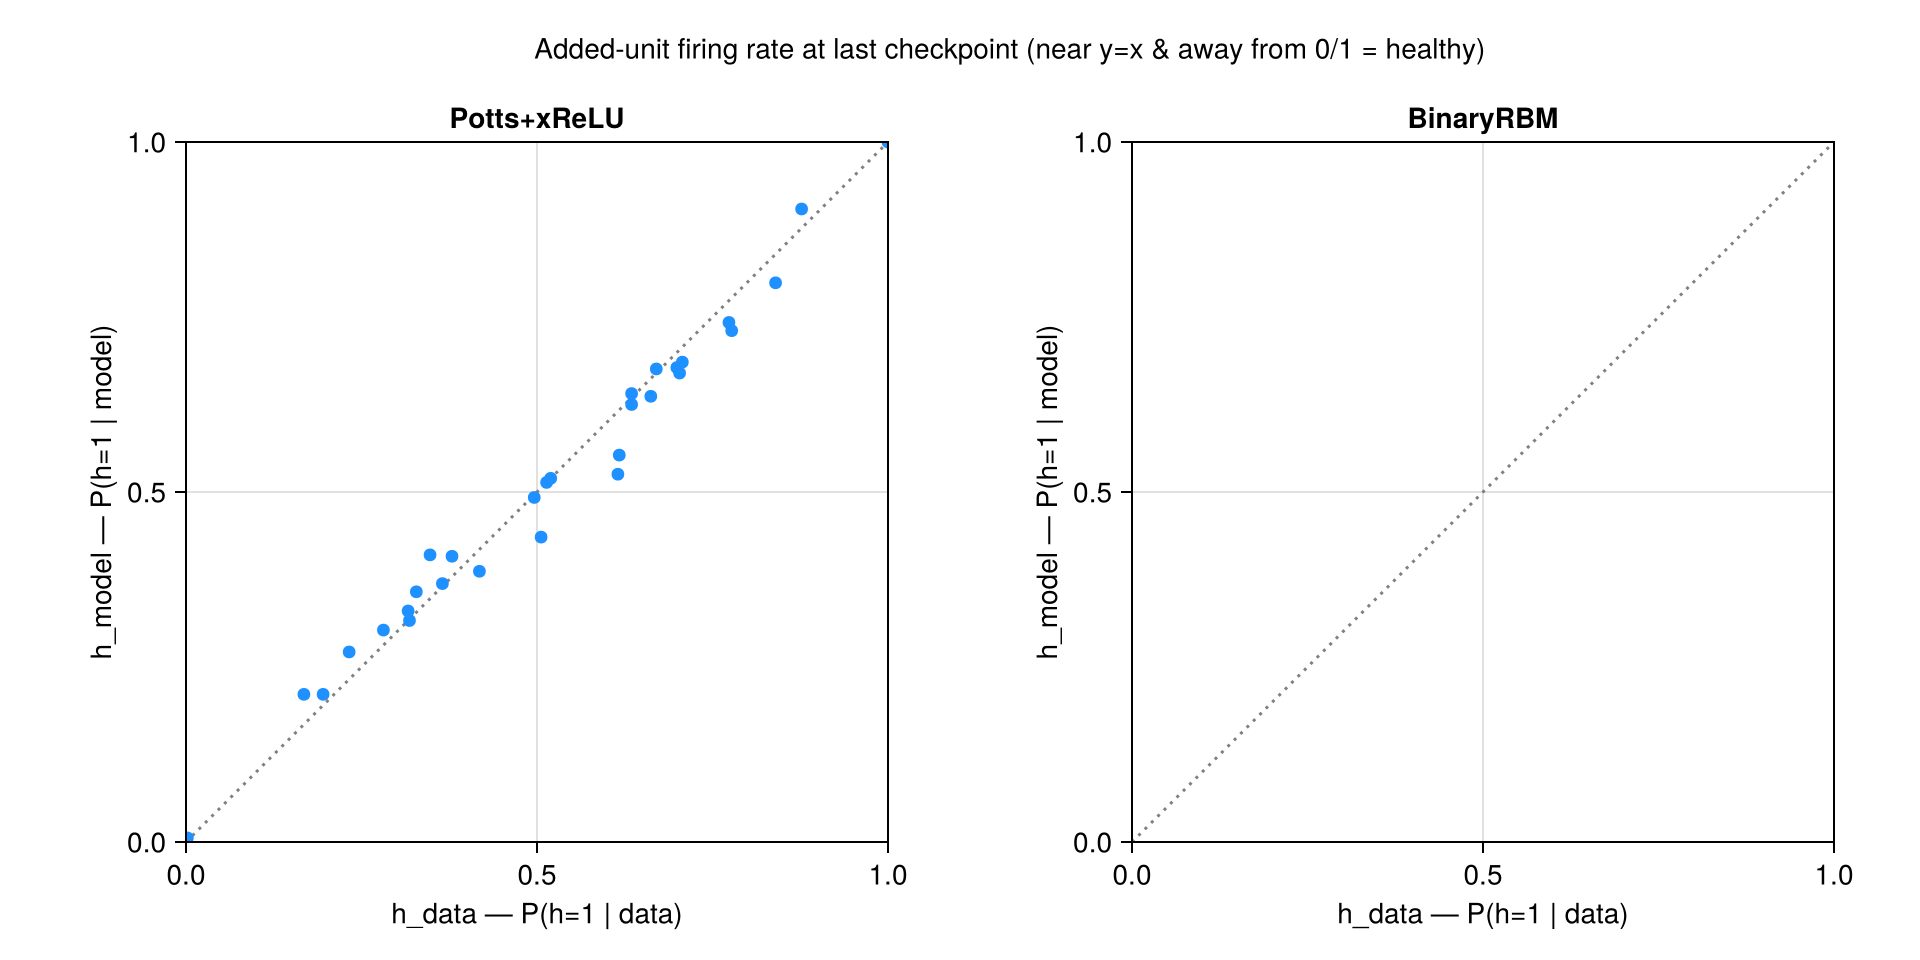
\includegraphics[width=0.55\linewidth]{figures/firing_rate.png}
\caption{Added units' firing rate $P(h=1)$ at the final training
checkpoint, data vs.\ model -- close to $y=x$ and away from the $0$/$1$
extremes, indicating healthy, non-degenerate activations.}
\label{fig:firing}
\end{figure}

\begin{figure}[H]
\centering
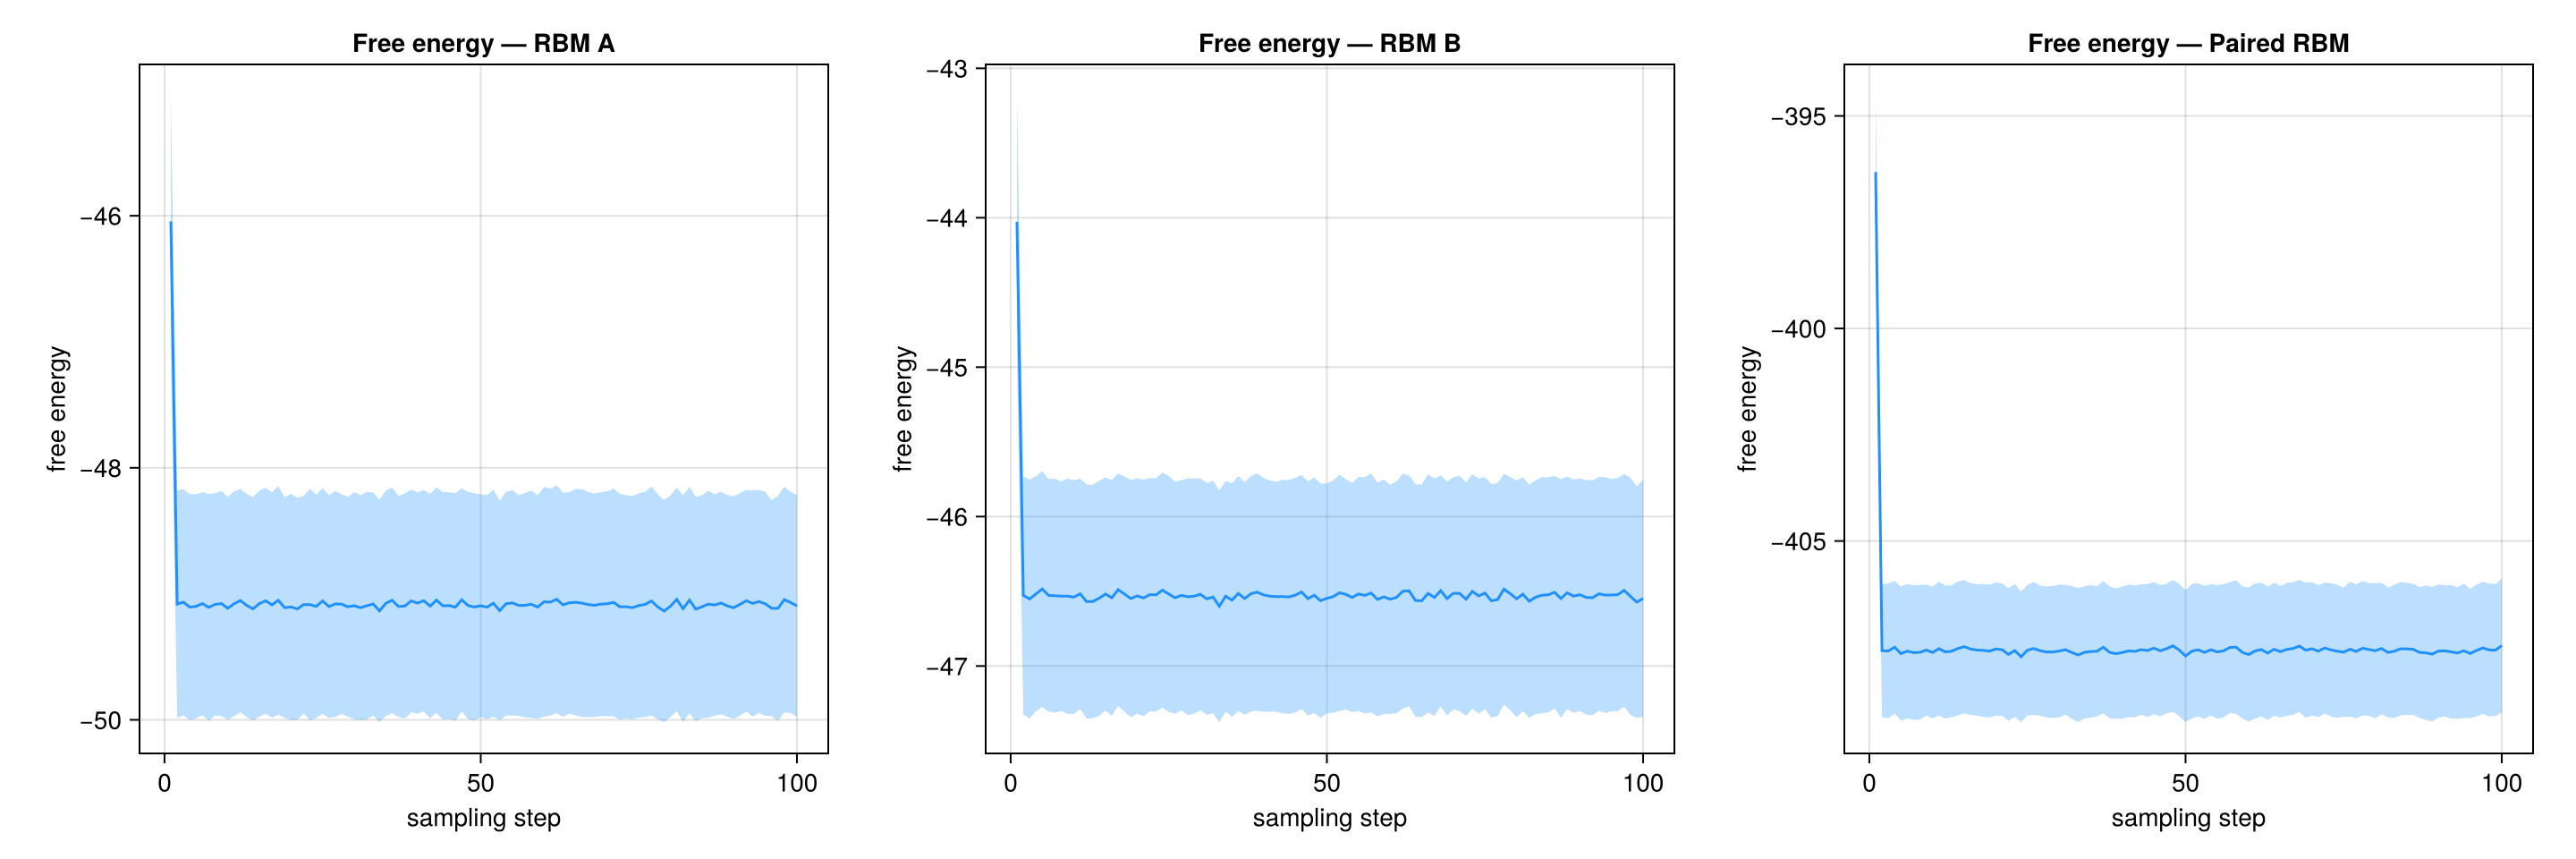
\includegraphics[width=0.55\linewidth]{figures/free_energy.png}
\caption{Free energy of the Gibbs chains vs.\ sweep count, averaged over
$5000$ chains. A plateau is reached well inside the $5000$-sweep burn-in
used for every equilibrium result below.}
\label{fig:freeenergy}
\end{figure}

The decisive test draws long, properly burnt-in Gibbs chains
(Fig.~\ref{fig:freeenergy} confirms equilibration well within budget).
Fig.~\ref{fig:blockhv} decomposes the resulting equilibrium samples by
hidden block: the frozen blocks reproduce the data well
($\rho=0.918$ for both $\langle h_Av_A\rangle$ and
$\langle h_Bv_B\rangle$), while the added units' correlation with the
\emph{full} visible layer tracks the data almost exactly
($\rho=0.996$ for $\langle h_{\mathrm{add}}v_{\mathrm{full}}\rangle$).

\begin{figure}[H]
\centering
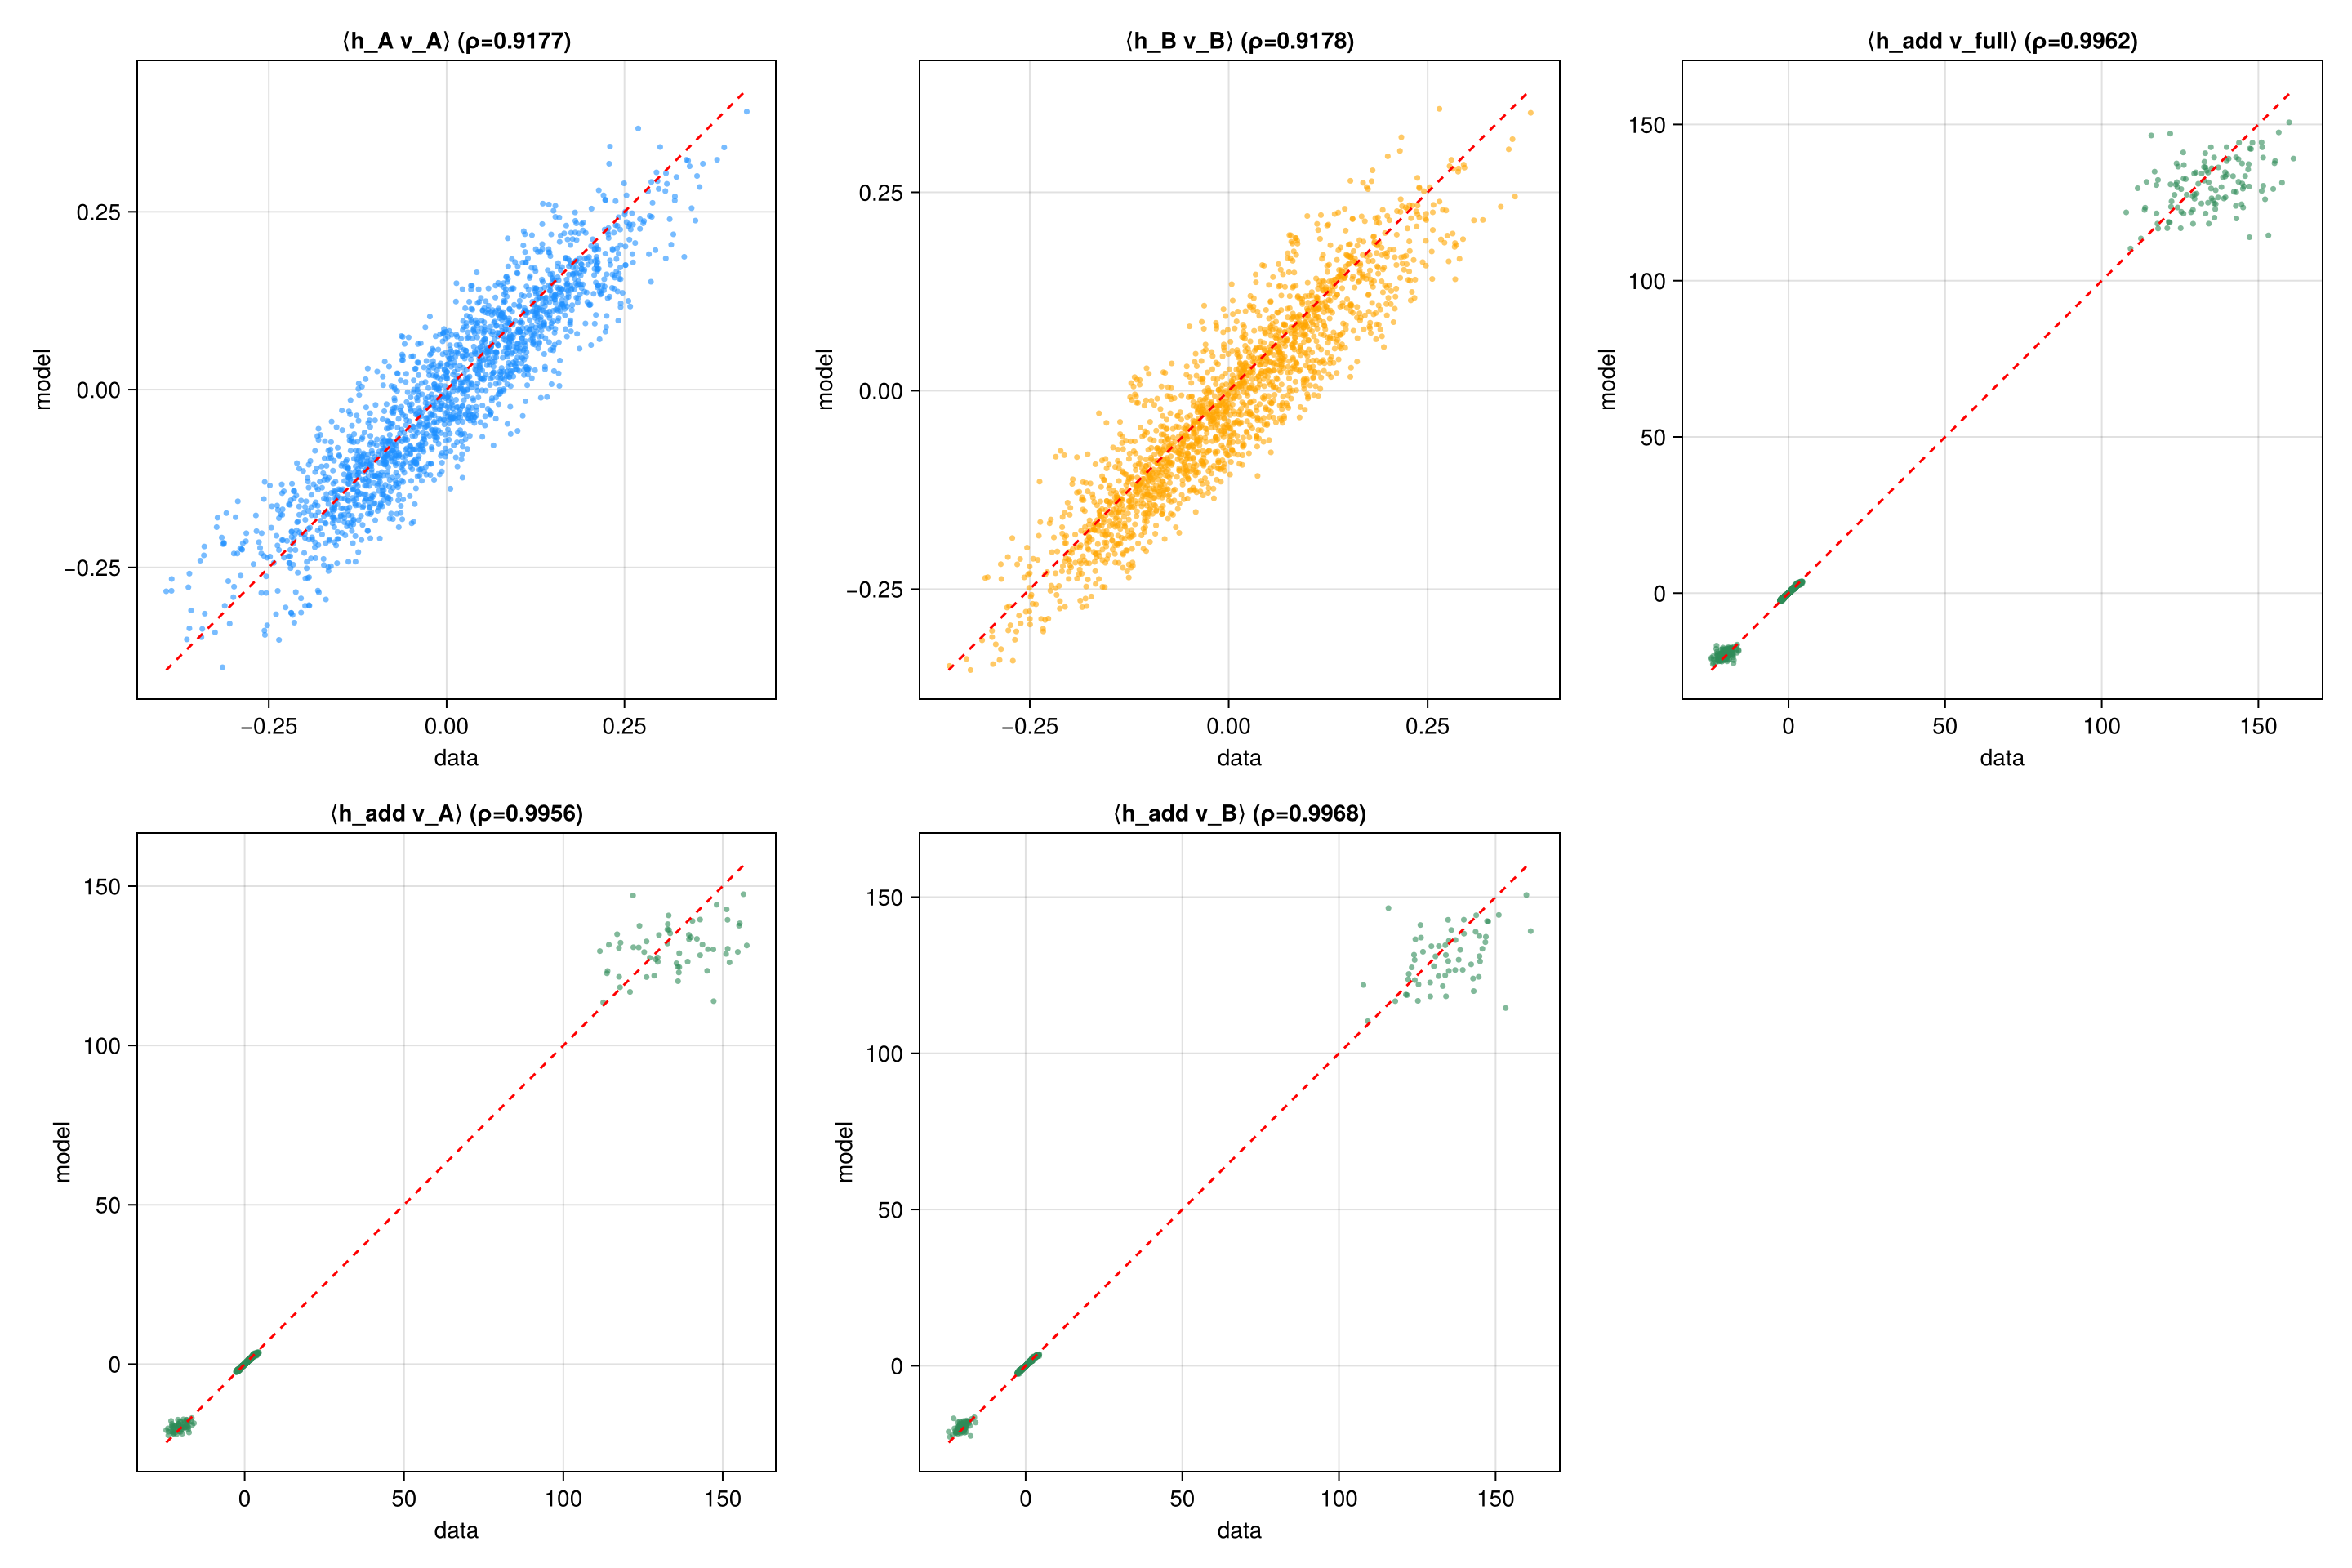
\includegraphics[width=0.78\linewidth]{figures/block_hv.png}
\caption{Data- vs.\ model-side $\langle hv\rangle$ from equilibrium Gibbs
samples, split by hidden block: frozen $A$--$A$/$B$--$B$ blocks, and the
added units against the full visible layer.}
\label{fig:blockhv}
\end{figure}

The central result is the direct comparison, at equilibrium, between the
recovered and true cross-family correlation matrices
(Fig.~\ref{fig:crosscorr}, Table~\ref{tab:headline}): the paired model
recovers $67\%$ of the $100$ strongest true couplings among its own $100$
strongest, against a $72\%$ ceiling from the finite-sample data and $10\%$
for the independent-RBM null; the whole-matrix correlation with $K$
reaches $r=0.837$ against a data ceiling of $r=0.845$ and an independent
baseline consistent with zero. Family-level intra-family correlation is
essentially preserved under pairing (off-diagonal $|{\rm corr}|$: family
$A$ $0.0565\to0.0606$, family $B$ $0.0455\to0.0503$).

\begin{table}[H]
\centering
\caption{Equilibrium validation against the true $K$ ($H_{\mathrm{add}}=30$,
seed $5$; $5000$ Gibbs chains, $5000$-sweep burn-in).}
\label{tab:headline}
\begin{tabular}{lccc}
\toprule
 & paired model & data (ceiling) & independent (null) \\
\midrule
top-100 overlap & 0.67 & 0.72 & 0.10 \\
corr.\ with $K$ & 0.837 & 0.845 & $-0.027$ \\
\bottomrule
\end{tabular}
\end{table}

\begin{figure}[H]
\centering
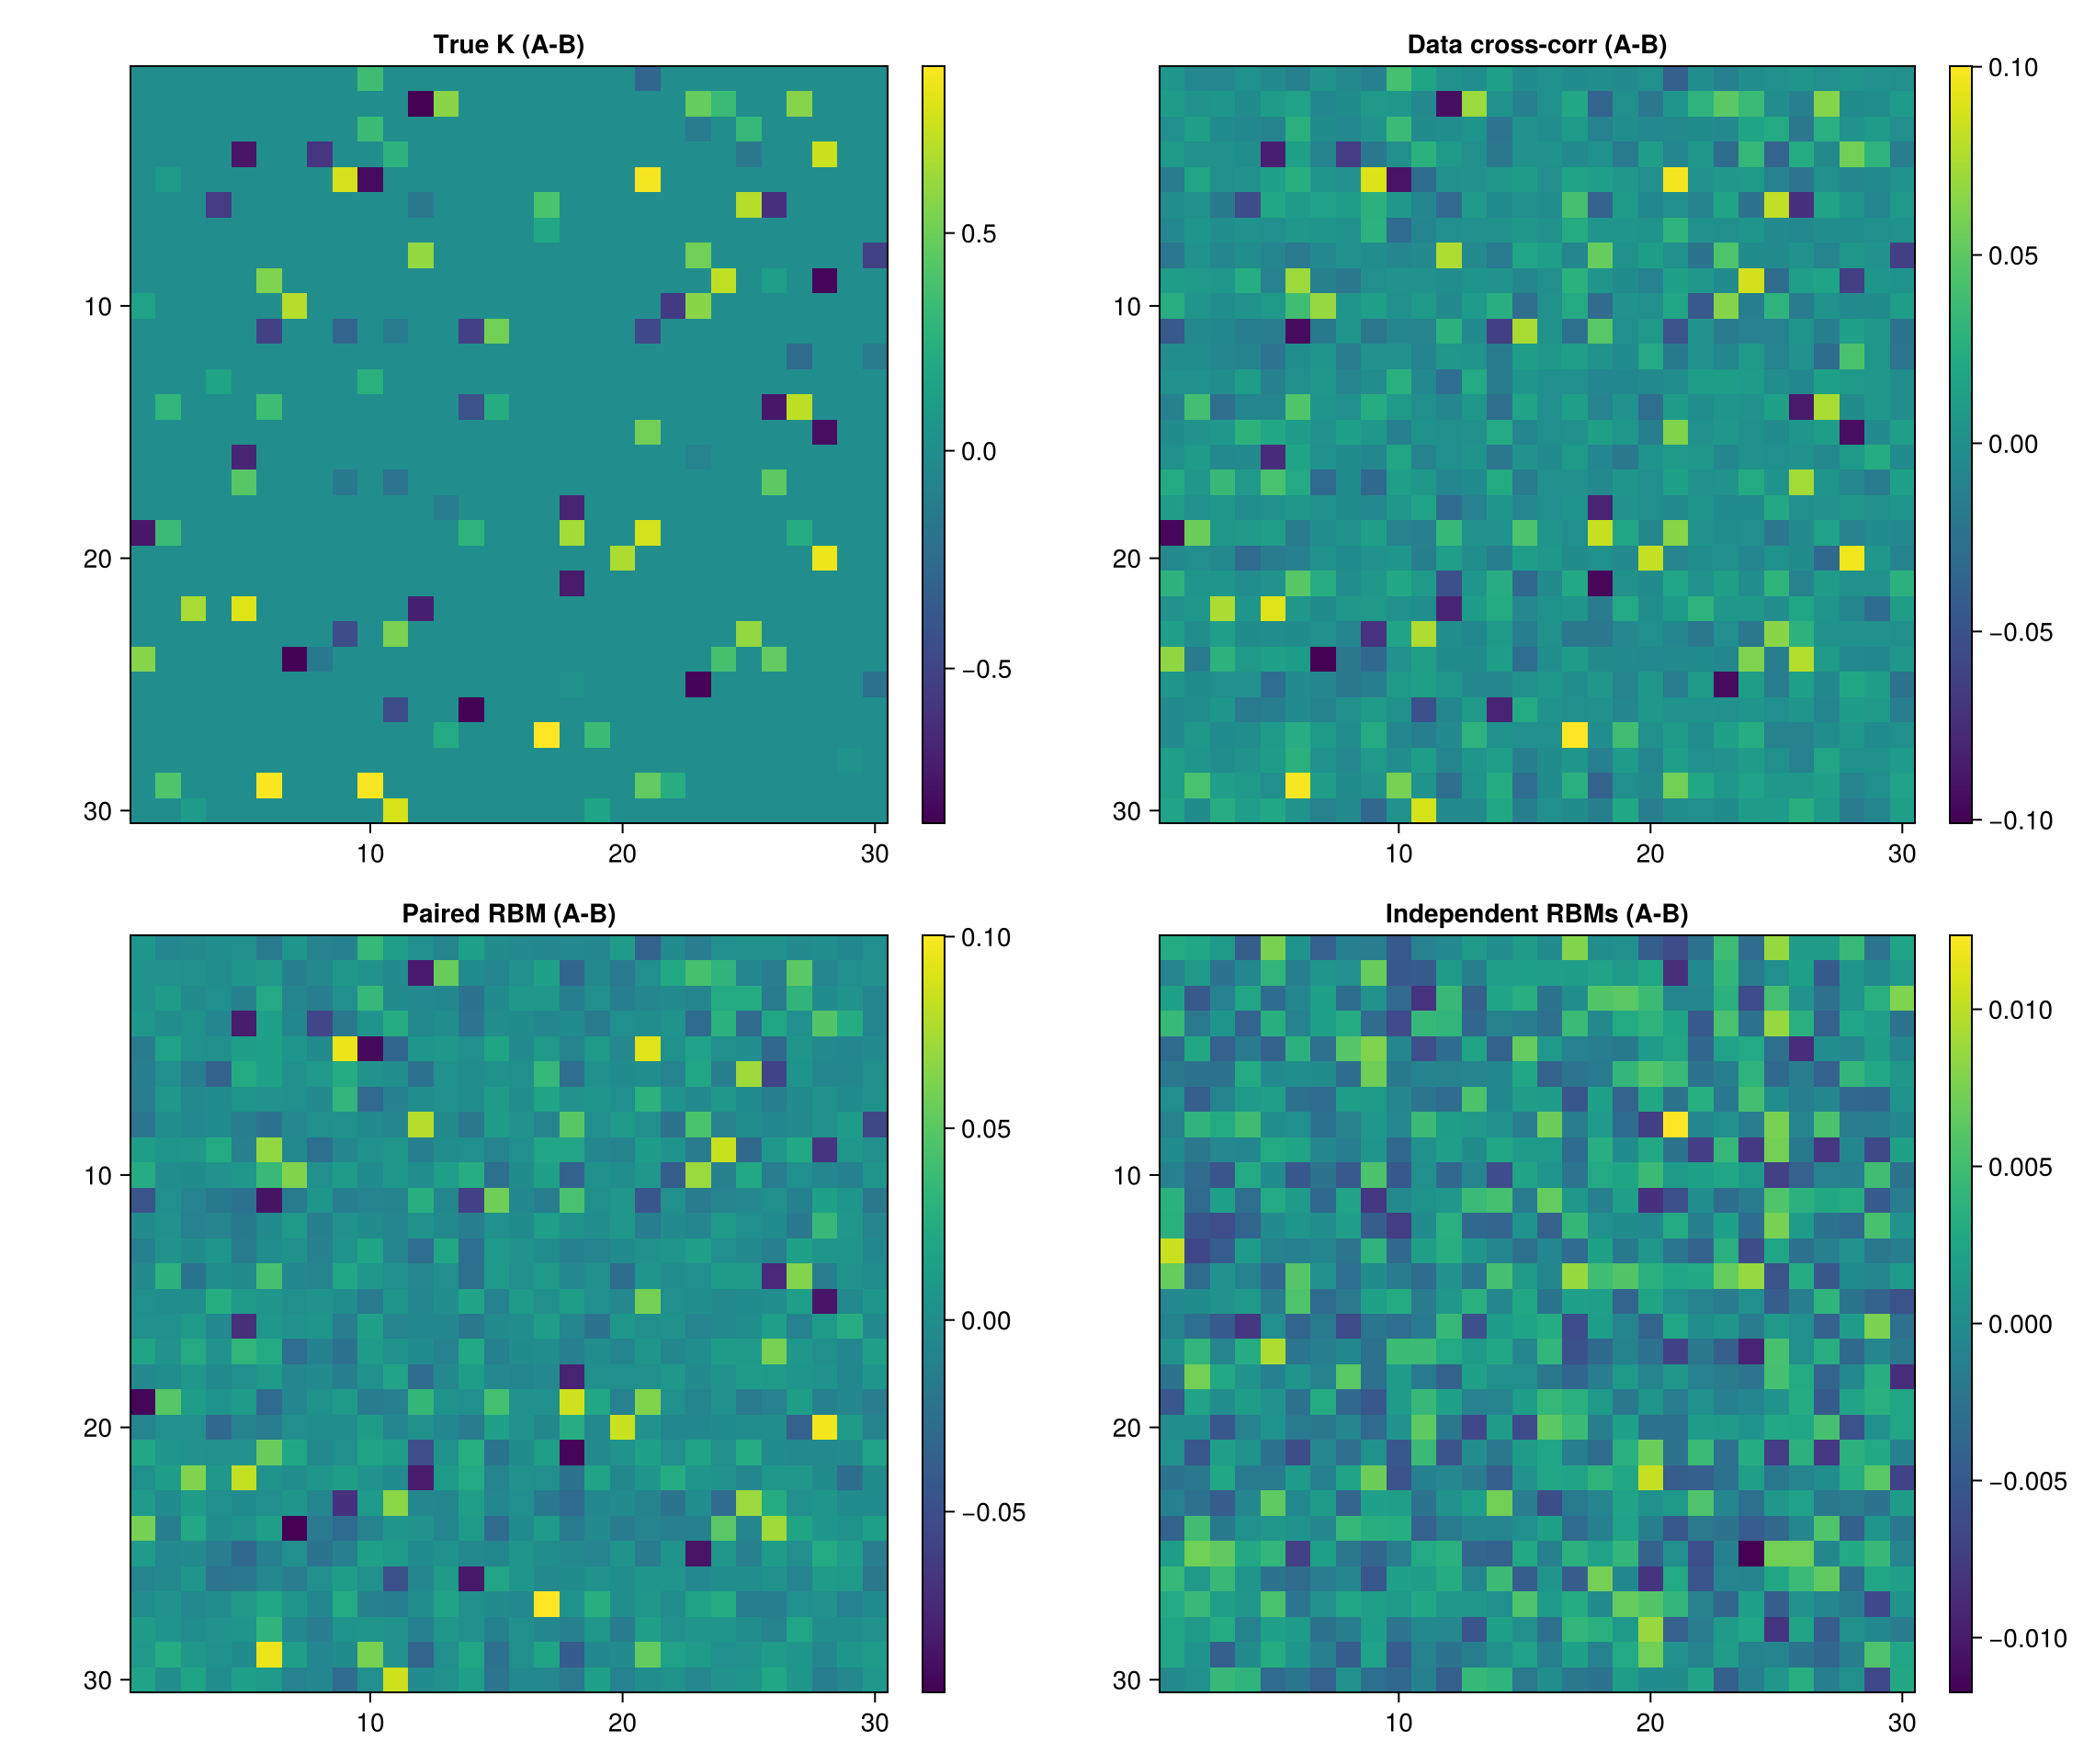
\includegraphics[width=0.85\linewidth]{figures/cross_corr.png}
\caption{Cross-family correlation matrices at equilibrium: true $K$,
empirical data correlation, correlation recovered by the paired model, and
correlation from two independent, uncoupled RBMs. The paired model
reproduces the sparse support of $K$ that is absent from the
independent baseline.}
\label{fig:crosscorr}
\end{figure}

\section{How many added units are needed? A capacity sweep}
\label{sec:hadd-sweep}

$H_{\mathrm{add}}=30$ above was a fixed, unjustified choice. Since the
added units are the sole channel for cross-family information, how many
are actually needed, and is there a cost -- not to recovery, but
elsewhere -- to using more or fewer?

\paragraph{Why the wide field range.} Answering this needs a diagnostic
finer than pairwise correlation: the single-site marginal
$\langle v_i\rangle$. Under a narrow field range ($h\in[-0.05,0.05]$,
tried first), the genuine site-to-site variation in $\langle v_i\rangle$
has standard deviation $\approx0.008$, smaller than the sampling error of
a mean over even $1000$ equilibrium samples ($\approx0.016$) -- an
observable that is structurally unusable regardless of model quality.
Widening the field to $h\in[-0.3,0.3]$ (Section~\ref{sec:model}) raises
the genuine signal to $\approx0.045$, comfortably above this noise floor,
without touching the coupling structure under study.

\paragraph{Two distinct failure modes.} With the wider field, the private
RBMs' $\langle v_i\rangle$ agreement is excellent ($\rho\approx0.99$) and
behaves like a noise-limited quantity. The \emph{paired} model's own
$\langle v_i\rangle$, however, does not: at $H_{\mathrm{add}}=30$ it
averages $\rho=0.263$ with a standard deviation of only $0.044$ across
$10$ independently trained seeds -- each seed drawing its own weight
initialisation, minibatch order, and $5000$-sweep equilibrium chains from
scratch. A quantity this reproducible across fully independent runs
cannot be sampling noise; it is a real, stable mismatch. The reason is
structural: only the added units can move a site's marginal away from what
its frozen private block predicts, but a hidden unit cannot encode a
correlation between two sites without also nudging each site's own
marginal -- the two effects share the same weight and are not separable.

\begin{figure}[H]
\centering
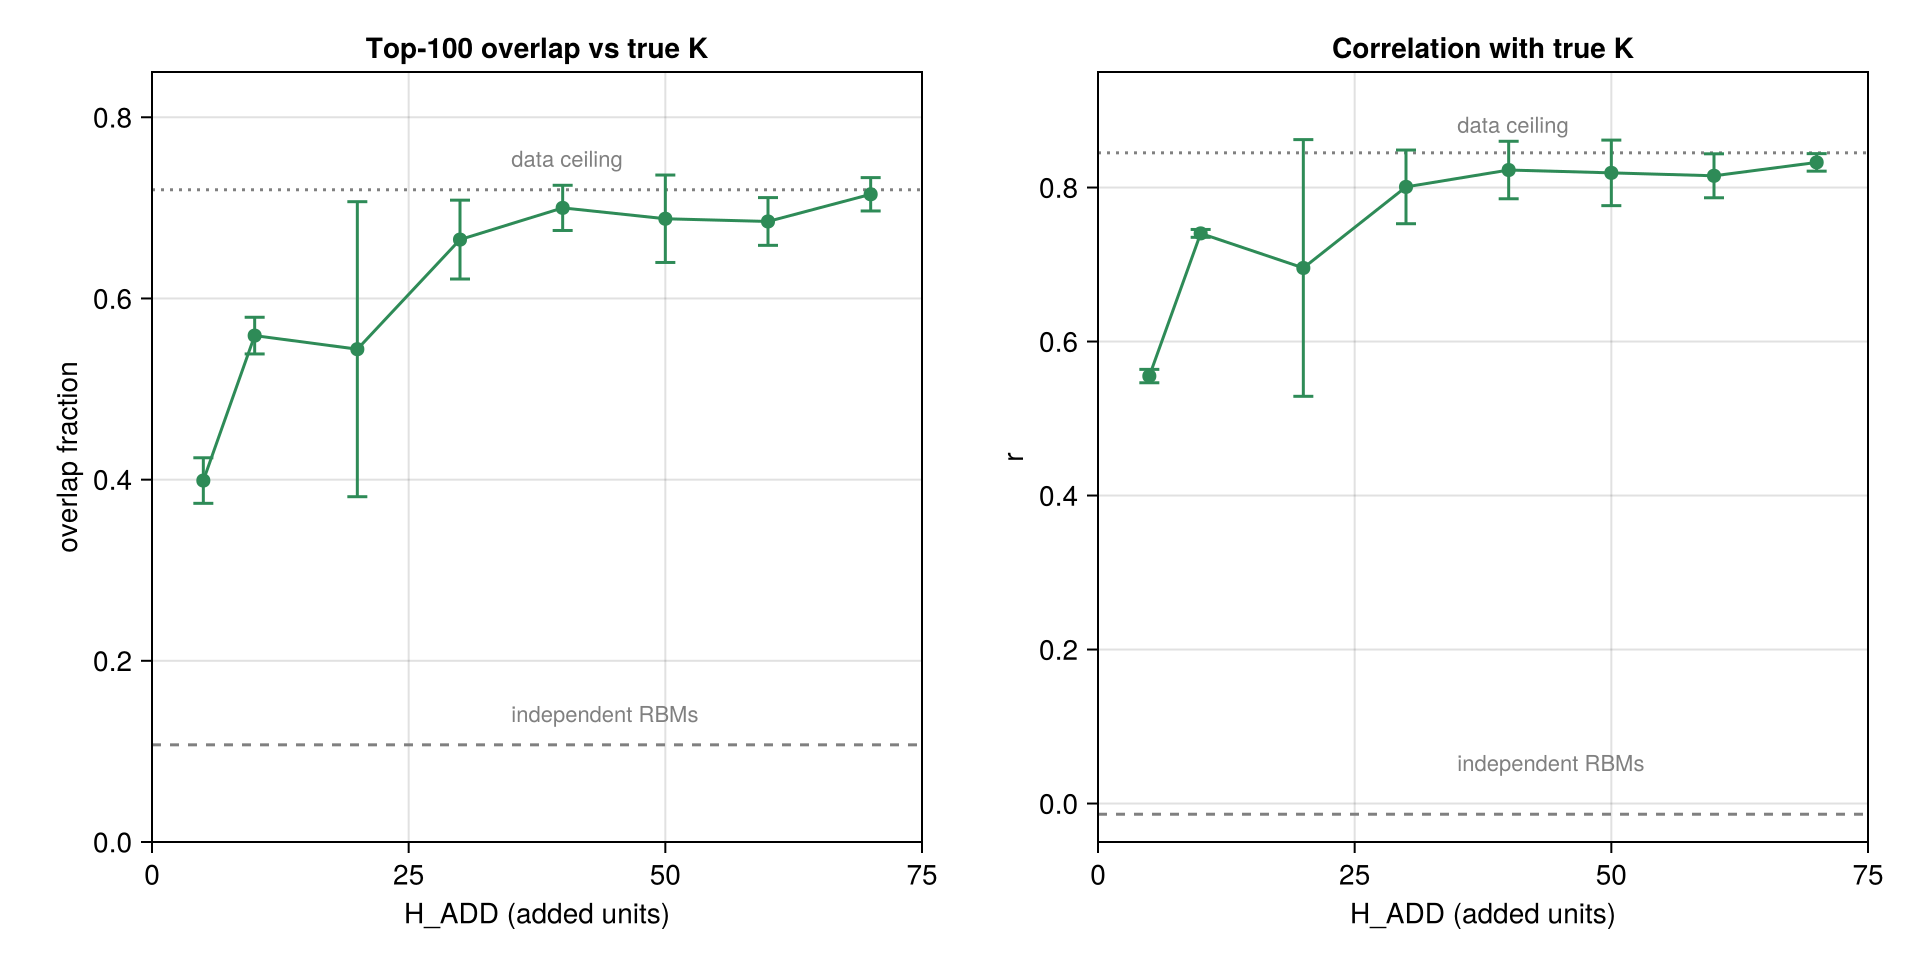
\includegraphics[width=0.9\linewidth]{figures/hadd_sweep_recovery.png}
\caption{Cross-family recovery vs.\ $H_{\mathrm{add}}$ (equilibrium Gibbs
samples, $N=5000$; mean $\pm$ standard deviation over $10$ independent
training seeds per point). Both metrics rise steeply up to
$H_{\mathrm{add}}\approx30$--$40$ and then plateau, within the run-to-run
spread, to $70$.}
\label{fig:haddrecovery}
\end{figure}

\paragraph{The sweep.} Repeating the full pipeline at
$H_{\mathrm{add}}\in\{5,10,20,30,40,50,60,70\}$, each with $10$ independent
random seeds (governing weight initialisation, minibatch order and the
persistent/equilibrium chains), gives $80$ independent runs
(Fig.~\ref{fig:haddrecovery}). Recovery rises steeply from
$H_{\mathrm{add}}=5$ (top-$100$ overlap $0.40\pm0.03$) through
$H_{\mathrm{add}}=20$ (overlap $0.54\pm0.16$ -- the one point with markedly
higher seed-to-seed spread, discussed below) to
$H_{\mathrm{add}}\approx40$--$70$ (overlap $0.68$--$0.72$, standard
deviation $\le0.05$, matching the $0.72$ data ceiling within noise):
thirty-to-forty added units already recover essentially everything
extractable from this coupling matrix, and the small seed-to-seed spread
from $H_{\mathrm{add}}=30$ on confirms the plateau is real, not a single
lucky run. At $H_{\mathrm{add}}=20$ specifically, $4$ of the $10$ seeds
land on a markedly worse optimum (overlap $0.26$--$0.49$) while the other
$6$ already reach $0.63$--$0.69$ -- consistent with this being the
narrowest part of the capacity transition, where whether a given run finds
the good solution is more a matter of chance than at either lower or
higher $H_{\mathrm{add}}$.

\begin{figure}[H]
\centering
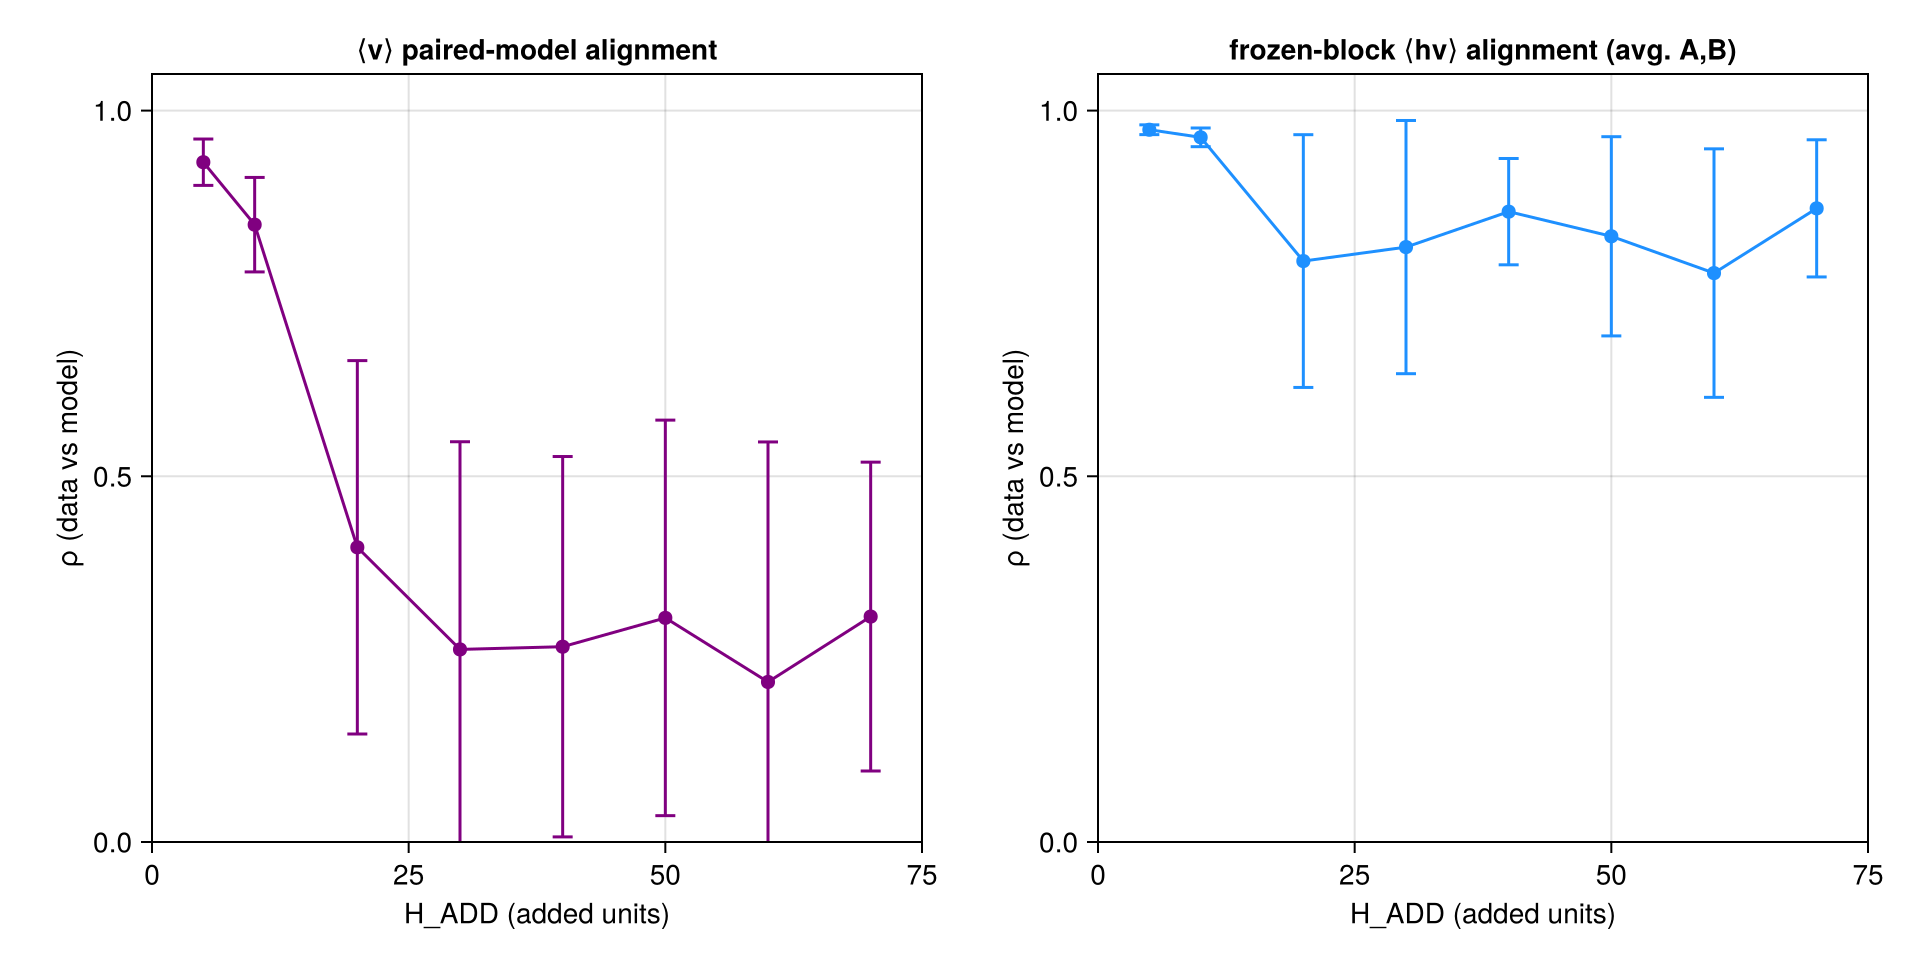
\includegraphics[width=0.9\linewidth]{figures/hadd_sweep_collateral.png}
\caption{Collateral effect on single-site statistics, same $80$ runs: paired
model's $\langle v\rangle$ agreement (left) and frozen-block $\langle
hv\rangle$ agreement, averaged over $A,B$ (right). Points are the mean over
$10$ seeds per $H_{\mathrm{add}}$; error bars are the standard deviation.}
\label{fig:haddcollateral}
\end{figure}

The collateral cost on single-site statistics (Fig.~\ref{fig:haddcollateral})
tells a monotone, not U-shaped, story here: agreement is high while
$H_{\mathrm{add}}$ is still too small to do much cross-family work
($H_{\mathrm{add}}=5$, mean $\langle v\rangle$ agreement $0.93$;
$H_{\mathrm{add}}=10$, mean $0.84$), drops sharply once the added units
start recovering real structure ($H_{\mathrm{add}}=20$, mean $0.40$), and
then sits on a noisy plateau around $0.22$--$0.31$ all the way out to
$H_{\mathrm{add}}=70$, with no sign of recovery at the largest sizes
tested. The frozen-block $\langle hv\rangle$ agreement (right panel) shows
the same shape with a shallower dip (from $\approx0.97$ at
$H_{\mathrm{add}}\le10$ to a $0.78$--$0.87$ plateau beyond it). This
contradicts what an earlier, shorter sweep at a ten-fold higher learning
rate and a third of the paired-training steps had suggested: there, the
same metric appeared to recover part-way back once $H_{\mathrm{add}}$ was
pushed well past the point needed for recovery. Training every
$H_{\mathrm{add}}$ here for the same $10\,000$ steps at $\mathrm{lr}=10^{-4}$
(long enough, with gradient clipping, to reach a stable plateau at every
size -- Fig.~\ref{fig:abcheck}) removes that apparent recovery: it was
most likely an artefact of the largest-$H_{\mathrm{add}}$ paired models
being relatively under-trained within a fixed, short step budget, not a
genuine benefit of spreading the same workload across more units.

\paragraph{Interpretation.} The collateral shift is not a transient,
undertraining artefact but a persistent cost of enabling any real
cross-family learning: below the capacity needed for recovery, the added
units simply are not doing much, so they cannot distort much either; once
they start doing genuine work, each family's own single-site statistics
take a corresponding, lasting hit that further over-provisioning does not
undo once training is run to full convergence. The practical lesson is
more sobering than a simple ``add more units'' fix: recovering
cross-family structure and keeping each subsystem's own statistics
undistorted are in real, structural tension in this construction, and no
amount of added-unit capacity resolves it on its own.

\section{Discussion}

A small, dedicated block of hidden units, added on top of two frozen,
independently trained models, recovers most of an otherwise hidden
inter-family coupling, confirmed directly against ground truth through
equilibrium sampling rather than training curves alone. The natural
whole-matrix correlation against a sparse $K$ is structurally capped well
below $1$ even for a perfect model (Table~\ref{tab:headline}'s
$0.845$ ceiling); reporting against that ceiling, not against $r=1$, is
essential. The capacity sweep (Section~\ref{sec:hadd-sweep}), run long
enough and with gradient clipping to reach full, stable convergence at
every size, revises the earlier picture from a shorter, higher-learning-rate
sweep: the tension between cross-family recovery and undistorted
single-site statistics does not resolve itself once enough capacity is
added -- it is structural, tracking how much genuine cross-family work the
added units are doing rather than how many of them there are. A further
methodological note follows from the same careful rerun: at this learning
rate and step count, unclipped gradients produced a late-training
instability in $54$ of the $80$ swept configurations, visible only as a
sharp, late collapse in pseudo-likelihood and a runaway added-unit weight
norm -- a reminder that training-time diagnostics need to be checked for
every configuration in a sweep, not spot-checked on a few, before their
downstream conclusions are trusted.

\end{document}
